% ======================================================================
% Paper B of the meander series: the tape machine and bounds on mu.
% Compile from this folder:  tectonic main.tex
% Sources (read-only): see the comment at the top of each section file and
% Appendix A. Numbers are quoted from the sources named there.
% Comments starting "% UNVERIFIED" mark statements the author could not confirm.
% ======================================================================
\documentclass[11pt]{article}
% Shared preamble for the meander paper series (papers A-D). Compile each paper with tectonic.
\usepackage[T1]{fontenc}
\usepackage[margin=1.15in]{geometry}
\usepackage{amsmath,amssymb,amsthm}
\usepackage{booktabs,array}
\usepackage{float}
\usepackage{tikz}
\usetikzlibrary{arrows.meta,decorations.pathmorphing,positioning}
\usepackage{pgfplots}
\pgfplotsset{compat=1.16}
\usepackage[colorlinks=true,linkcolor=blue!50!black,citecolor=blue!50!black,urlcolor=blue!50!black]{hyperref}

\newtheorem{theorem}{Theorem}
\newtheorem{proposition}[theorem]{Proposition}
\newtheorem{lemma}[theorem]{Lemma}
\newtheorem{corollary}[theorem]{Corollary}
\newtheorem{conjecture}[theorem]{Conjecture}
\theoremstyle{definition}
\newtheorem{definition}[theorem]{Definition}
\theoremstyle{remark}
\newtheorem*{remark}{Remark}

\emergencystretch=2em
\raggedbottom

% Tapes of the tape machine. Write -{}- for a double minus inside \tape{...} to avoid the
% typewriter dash ligature.
\newcommand{\tape}[1]{\texttt{#1}}
\newcommand{\hd}[1]{\texttt{[#1]}}

% Series line under the title.
\newcommand{\seriesline}[1]{\par\smallskip{\small\itshape Meander numbers: growth rate and exponent. #1}}

% The running example (order 3): upper arches (1,2), (3,6), (4,5); lower arches (1,6), (2,5), (3,4).
\newcommand{\meanderroad}{%
  \draw (1,0) arc[start angle=180,end angle=0,radius=0.5];
  \draw (3,0) arc[start angle=180,end angle=0,radius=1.5];
  \draw (4,0) arc[start angle=180,end angle=0,radius=0.5];
  \draw (1,0) arc[start angle=180,end angle=360,radius=2.5];
  \draw (2,0) arc[start angle=180,end angle=360,radius=1.5];
  \draw (3,0) arc[start angle=180,end angle=360,radius=0.5];
}
\newcommand{\meanderfigure}{%
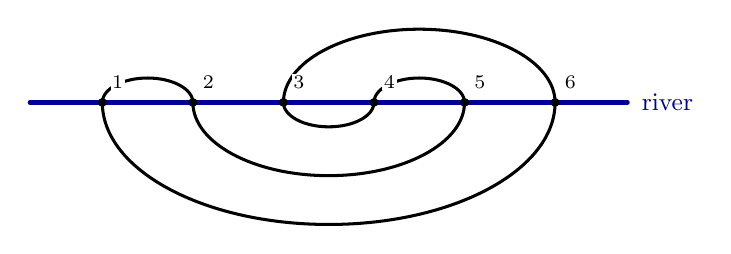
\begin{tikzpicture}[x=1.15cm,y=0.62cm,line cap=round]
  \draw[blue!60!black,line width=1.6pt] (0.2,0)--(6.8,0);
  \node[blue!60!black,anchor=west] at (6.85,0) {\small river};
  \begin{scope}[line width=1.1pt]\meanderroad\end{scope}
  \foreach \k in {1,...,6} {\fill (\k,0) circle[radius=1.6pt]; \node[fill=white,inner sep=0.6pt,font=\scriptsize] at (\k+0.17,0.42) {\k};}
\end{tikzpicture}}

% The series. Each paper cites the others as \cite{PaperA} etc.


% Local notation for this paper (does not change ../common).
\newcommand{\Lm}{\mathord{\leftarrow}}      % move: head left
\newcommand{\Rm}{\mathord{\rightarrow}}     % move: head right
\newcommand{\Sone}{\mathsf{S}_1}
\newcommand{\Stwo}{\mathsf{S}_2}
\newcommand{\Sthree}{\mathsf{S}_3}
\newcommand{\Mm}{\mathsf{M}}                % move: merge
\newcommand{\cls}{\mathcal{C}}              % class of tapes reached from the root
\newcommand{\cpl}[1]{\overline{#1}}         % complement of a tape
\newtheorem*{theoremF}{Theorem F}
% Float spacing for this paper.
\setlength{\textfloatsep}{14pt plus 3pt minus 3pt}
\setlength{\floatsep}{12pt plus 2pt minus 2pt}
\setlength{\intextsep}{12pt plus 2pt minus 2pt}
\def\UrlBreaks{\do\/\do\_\do\.}  % break file paths at / _ .

% One tape drawn as a row of boxes: #1 shift, #2 comma list of + and -, #3 head index.
\newcommand{\tp}[3]{%
  \begin{scope}[shift={#1}]
  \foreach \c [count=\i] in {#2} {
    \ifnum\i=#3\relax
      \draw[line width=0.9pt,fill=red!13] ({(\i-1)*0.36},-0.18) rectangle ++(0.36,0.36);
    \else
      \draw[line width=0.4pt] ({(\i-1)*0.36},-0.18) rectangle ++(0.36,0.36);
    \fi
    \node[font=\small,inner sep=0pt] at ({(\i-0.5)*0.36},0) {$\c$};
  }
  \end{scope}}

\begin{document}

\title{The tape machine and bounds on the growth rate of meanders\seriesline{Paper B.}}
\author{Carl Johan Ragnarsson}
\date{Draft of October 25, 2026}
\maketitle

% Abstract. Numbers: ledger/facts.json (muLower, muUpper); 1228_combined_lower/FINAL.md; 1201_upper_structures/FINAL.md.
\begin{abstract}
A meander of order $n$ is a closed road that crosses a straight river $2n$ times without crossing itself. Their number
$M_n$ grows like $\mu^n$, and the growth rate $\mu$ is estimated numerically at $12.2629$. We prove
\[ 12.2191 \;\le\; \mu \;\le\; 12.2970 . \]
The best bounds in a journal are $11.380$ and $12.901$. Both bounds use the tape machine: a meander is read from left
to right, one crossing at a time, and the state between two crossings is a word in $+$ and $-$ with a marked letter,
the head. Each crossing changes only the head and its two neighbors. Meanders of order $n$ are exactly the closed
walks of $2n-2$ moves from the tape $+[-]+$ back to itself. For the upper bound we give two positive weights to every
tape and a positive factor to every move, with reciprocal factors on a move and its reverse, and check a finite list of
$2{,}097{,}152$ inequalities in exact rational arithmetic; together they show that the number of closed walks grows
by at most a factor $3.50670$ per move. For the lower bound we construct a random rule for choosing moves that is stationary
and on average does not let the tape grow; its entropy is at least $1.2515$ per move, and a counting argument turns
this into $\mu\ge e^{2\cdot 1.2515}$. Each certificate was checked again by
a second, separately written program; for the lower bound, part of this second check covers a sample of the
equations rather than all of them. The arguments were read independently. We also describe what limits both
methods. All code was written using Claude (Opus 5.5) or Codex (Sol 5.1) with active review and guidance throughout.
\end{abstract}

% Section 1. Sources: 607_bounds_paper/paper.tex (history, problem statement), ledger/STATE.md and
% ledger/facts.json (rows mu upper, mu lower), 1201_upper_structures/runs/r9_run2_verify.json (exact R),
% 1251_referee_upper_12297/FINAL.md, 1228_combined_lower/FINAL.md, 1252/1253 FINAL.md.
%%%%%%%%%%%%%%%%%%%%%%%%%%%%%%%%%%%%%%%%%%%%%%%%%%%%%%%%%%%%%%%%%%%%%%%%
\section{Introduction}\label{sec:intro}
%%%%%%%%%%%%%%%%%%%%%%%%%%%%%%%%%%%%%%%%%%%%%%%%%%%%%%%%%%%%%%%%%%%%%%%%

\subsection{The problem}

A meander of order $n$ is a closed road that crosses a straight river $2n$ times and never crosses itself. Two drawings
are the same meander if one can be deformed into the other without changing the order of the crossings. Their number
is $M_n$:
\[ M_1, M_2, \ldots \;=\; 1,\ 2,\ 8,\ 42,\ 262,\ 1828,\ 13820,\ 110954,\ \ldots \]
Figure~\ref{fig:cut} shows one of the $8$ meanders of order $3$; it is the running example of this paper. No formula
for $M_n$ is known. The limit $\mu=\lim M_n^{1/n}$ exists~\cite{AP}, and series analysis of the exact counts gives
$\mu\approx 12.262874$~\cite{JG}. This value is a numerical estimate, not a proved bound. Paper~A of this series~\cite{PaperA} explains why the
problem is hard and what is expected; Paper~C~\cite{PaperC} studies the factor $M_n/\mu^n$ and Paper~D~\cite{PaperD}
a continuum model. This paper proves bounds on $\mu$.

\begin{figure}[htb]
\centering
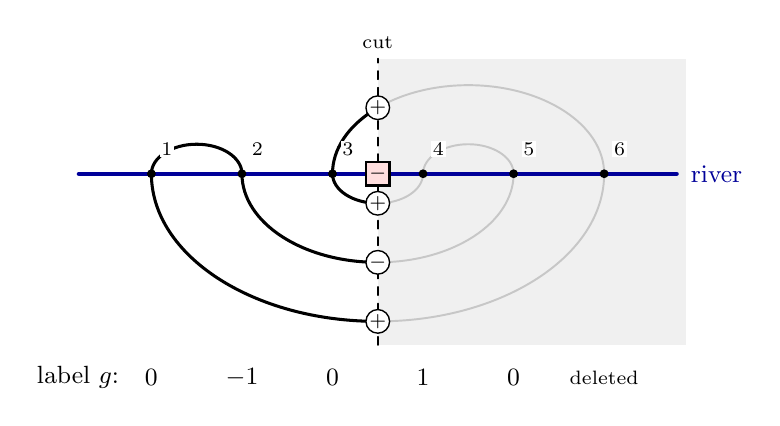
\begin{tikzpicture}[x=1.15cm,y=0.75cm,line cap=round]
  \fill[black!6] (3.5,-2.9) rectangle (6.9,1.95);
  \draw[blue!60!black,line width=1.6pt] (0.2,0)--(6.8,0);
  \node[blue!60!black,anchor=west] at (6.85,0) {\small river};
  \begin{scope}[black!22,line width=0.7pt]\meanderroad\end{scope}
  \begin{scope}\clip (0.2,-2.9) rectangle (3.5,1.95);
    \begin{scope}[line width=1.1pt]\meanderroad\end{scope}\end{scope}
  \draw[dashed,line width=0.6pt] (3.5,-2.9)--(3.5,1.95);
  \node[font=\scriptsize,anchor=south] at (3.5,1.95) {cut};
  \foreach \k in {1,...,6} {\fill (\k,0) circle[radius=1.6pt];
    \node[fill=white,inner sep=0.6pt,font=\scriptsize] at (\k+0.17,0.42) {\k};}
  % signs of the strands met by the cut, bottom to top: + - + [-] +
  \foreach \yy/\s in {-2.5/+,-1.5/-,-0.5/+,1.118/+} {
    \draw[fill=white,line width=0.5pt] (3.5,\yy) circle[radius=0.15cm];
    \node[font=\scriptsize,inner sep=0pt] at (3.5,\yy) {$\s$};}
  \draw[fill=red!13,line width=0.8pt] (3.5,0) ++(-0.15cm,-0.15cm) rectangle ++(0.3cm,0.3cm);
  \node[font=\scriptsize,inner sep=0pt] at (3.5,0) {$-$};
  % labels of the crossings
  \node[anchor=east,font=\small] at (0.75,-3.45) {label $g$:};
  \foreach \k/\g in {1/0,2/-1,3/0,4/1,5/0} {\node[font=\small] at (\k,-3.45) {$\g$};}
  \node[font=\scriptsize] at (6,-3.45) {deleted};
\end{tikzpicture}

\smallskip
{\small tape $+-+[-]+$\qquad stacks $\sigma=(0,-1,0)$, $\tau=(0)$\\
gap numbers from bottom to top $-1,0,-1,0,-1,0$}
\caption{The running example, a meander of order $3$, with the cut after crossing $3$ and the part to the right covered
(gray). The cut meets three unfinished arches below the river, the river, and one unfinished arch above. Reading their
signs from bottom to top gives the tape; the square marks the head on the river. Below the drawing are the labels $g$
of the crossings; crossing $6$ is deleted when labels are assigned. Labels, stacks, gap numbers and tapes are defined
in Section~\ref{sec:tape}.}
\label{fig:cut}
\end{figure}

\subsection{Previous bounds and the main result}

Albert and Paterson proved $11.380\le\mu\le12.901$ in 2005~\cite{AP}. In 2026 Fox released code with certified bounds
$11.6080\le\mu\le12.6319$~\cite{Fox}, and Caroppo, Da~Lozzo, Di~Battista and Vihrovs stated $\mu\le12.806$ in a
preprint~\cite{CDDV}. Earlier in this project a weight method on an encoding of meanders by bracket words gave
$12.0535\le\mu\le12.4147$~\cite{BoundsPaper}. Table~\ref{tab:history} and Figure~\ref{fig:history} collect these
bounds. All bounds in the table are proved; the value $12.2629$ is not.

\begin{theorem}\label{thm:main}
Let $R_+$ be the rational number stored in the upper-bound certificate of Section~\ref{sec:upper}; its numerator and
denominator have $111$ digits, and $R_+=3.50669842637333\ldots<3506698427/10^9$. Then
\[ \frac{6109550428547}{500000000000} \;=\; 12.219100857094 \;\le\; \mu \;\le\; R_+^2 \;=\; 12.29693385352921289818\ldots \]
In particular $12.2191\le\mu\le12.2970$. Moreover $M_n\le R_+^{\,2n-2}$ for every $n\ge1$.
\end{theorem}

The interval has width $0.0778$ and contains the estimate $12.2629$, which lies $0.0438$ above the lower bound and
$0.0341$ below the upper bound.
% Arithmetic: 12.262874-12.219100857 = 0.043773; 12.296933854-12.262874 = 0.034060; width 0.077833 (1228 FINAL: 0.077832997).

\begin{table}[htb]
\centering
\begin{tabular}{llll}
\toprule
lower bound & upper bound & source & method \\
\midrule
$11.380$ & $12.901$ & Albert and Paterson, 2005~\cite{AP} & subclasses; clusters\\
$11.6080$ & $12.6319$ & Fox, 2026~\cite{Fox} & selected states; forgetting\\
 & $12.806$ & Caroppo et al., 2026~\cite{CDDV} & (not examined here)\\
$12.0535$ & $12.4147$ & this project, earlier~\cite{BoundsPaper} & window weights\\
$12.2191$ & $12.2970$ & this paper & tape machine\\
\bottomrule
\end{tabular}
\caption{Bounds on $\mu$. The last column names the method of each source in a few words. The numerical estimate
is $12.2629$.}
\label{tab:history}
\end{table}

\begin{figure}[htb]
\centering
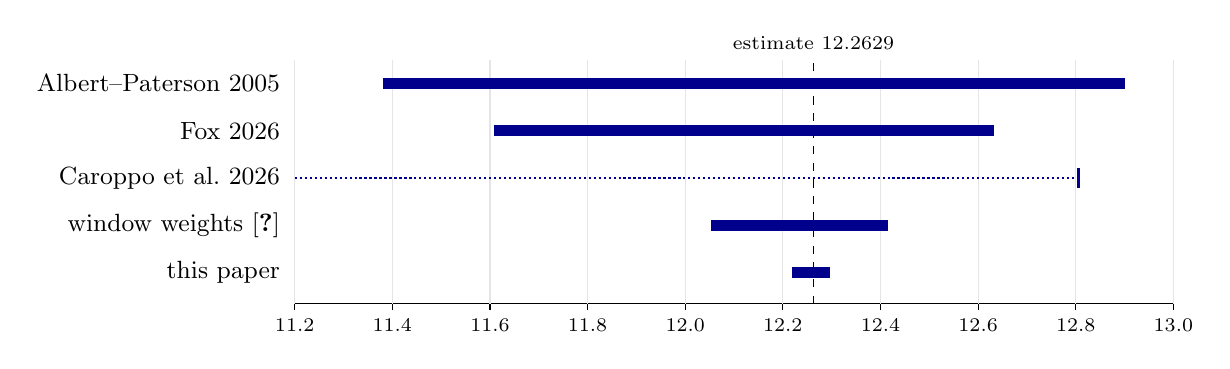
\begin{tikzpicture}[x=6.2cm,y=0.5cm]
  % axis from 11.2 to 13.0
  \draw[line width=0.5pt] (11.2,-5.6)--(13.0,-5.6);
  \foreach \v in {11.2,11.4,11.6,11.8,12.0,12.2,12.4,12.6,12.8,13.0} {
    \draw (\v,-5.6)--(\v,-5.75); \node[font=\scriptsize,anchor=north] at (\v,-5.75) {\v};
    \draw[black!10] (\v,-5.6)--(\v,0.6);
  }
  \draw[dashed,line width=0.6pt] (12.2629,-5.6)--(12.2629,0.6);
  \node[font=\scriptsize,anchor=south] at (12.2629,0.6) {estimate $12.2629$};
  % rows
  \foreach \lo/\hi/\y/\name in {11.380/12.901/0/{Albert--Paterson 2005},11.6080/12.6319/-1.2/{Fox 2026},12.0535/12.4147/-3.6/{window weights~\cite{BoundsPaper}},12.2191/12.2970/-4.8/{this paper}} {
    \draw[line width=4pt,blue!55!black] (\lo,\y)--(\hi,\y);
    \node[font=\small,anchor=east] at (11.19,\y) {\name};
  }
  \draw[densely dotted,line width=0.8pt,blue!55!black] (11.2,-2.4)--(12.806,-2.4);
  \draw[line width=1.2pt,blue!55!black] (12.806,-2.65)--(12.806,-2.15);
  \node[font=\small,anchor=east] at (11.19,-2.4) {Caroppo et al.\ 2026};
\end{tikzpicture}
\caption{The bounds of Table~\ref{tab:history} as intervals. The third row has an upper bound only. The dashed line is the
numerical estimate, which is not a bound.}
\label{fig:history}
\end{figure}

\subsection{The methods in outline}

\emph{The tape machine} (Section~\ref{sec:tape}). Cover a meander with a sheet of paper and slide the sheet to the
right, uncovering the crossings one at a time from the left. Where the sheet stops, its edge meets unfinished pieces of
road below the river, the river, and unfinished pieces above. Each of them gets a sign, $+$ or $-$, by a rule
explained in Section~\ref{sec:tape}. Read from bottom to top, the signs form a word, the \emph{tape}, and the letter
of the river is marked as the \emph{head}. Uncovering one more crossing is a \emph{move}: it changes the tape only at
the head and its two neighbors. Meanders of order $n$ correspond exactly to the sequences of $2n-2$ moves that start
and end at the tape $+[-]+$ (the \emph{closed walks}). Tapes can be arbitrarily long, but every move is local, and both
methods use this.

\emph{The upper bound} (Sections~\ref{sec:weights} and~\ref{sec:upper}). If every tape has a positive weight and the
tapes one move later (its \emph{successors}) weigh at most $R$ times as much in total, then there are at most $R^t$
closed walks of $t$ moves. Since a meander of order $n$ takes $2n-2$ moves, this gives $\mu\le R^2$. We use a sharper
form of this test: each tape has a forward and a backward weight, and each move carries a factor whose reciprocal is
carried by the reverse move. The weights are built so that the ratios entering the test depend only on the letters
near the head, so a finite list of cases covers all tapes. The finite data together with the exact check of these cases is the
\emph{certificate}; here and below, a \emph{certified} bound is one proved by such a check.

\emph{The lower bound} (Sections~\ref{sec:flows} and~\ref{sec:lower}). Consider a random rule for the next move that
is stationary, so that the tape seen from the head looks statistically the same at all times, and that on average
neither lengthens the tape nor moves the head toward one end. Such a rule produces about $e^{ht}$ different sequences
of $t$ moves, where $h$ is its entropy per move, and each of them can be completed to a closed walk with few extra
moves. This gives $\mu\ge e^{2h}$. The certificate is such a rule, written as an exact solution of a finite system of
linear equations.

\subsection{Status of the results}

The tape machine (Theorem~\ref{thm:tape}) and both certificates are new in this project. The bijection was proved in
the project, checked in a separate independent reading, and confirmed by counting closed walks up to order $15$. The
upper certificate was checked in exact rational arithmetic by its own checker and by a second checker written
independently from a separate statement of the theorem; that independent reading also re-proved each step from the
certificate to the bound. The lower certificate rests on a theorem about stationary random rules (Theorem~F in
Section~\ref{sec:flows}) and on four constructions that keep the rule exactly stationary; each of these arguments was
re-derived in a separate independent reading, and the computation was reproduced and recomputed with independently
written code. One part of the lower check is a sample, not a complete replay: the linear equations that express
stationarity for the two largest windows hold by construction and were confirmed only on samples
(Section~\ref{sec:checks}). Nothing has been reviewed outside the project, and no proof assistant was used. Programs,
proofs and certificates are in the project repository~\cite{Repo}; Appendix~\ref{app:where} lists where each proof is.

We have not found the tape machine in the literature. Our search was limited, and the general idea of reading a
meander from left to right while keeping the unfinished arches in two stacks is classical; see~\cite{Jensen} for a transfer matrix method of this
kind.

% Section 2. Sources: 637_rung2_matrix_product/PROOF.md section 1 (Proposition T) and FINAL.md;
% 677_tape_bijection_review/REVIEW.md; 607_bounds_paper/paper_word.tex Appendix A (labels, stacks, words) and
% Appendix B (linear completion); 805_entropy_certificates/PROOF.md section 1.2 step 3 (Lemmas R and B);
% 641_tape_window_bounds/PROOF.md section 0 (class C); web/src/meandric/tapeMachine.ts and TapeMachineWriteup.tsx
% (rules as implemented, gap numbers, picture of a move). Counts: 1251 FINAL (n <= 9), 1252 FINAL EY6 (n <= 15).
% The worked examples were re-derived with a small script written for this paper (rules of tapeMachine.ts).
%%%%%%%%%%%%%%%%%%%%%%%%%%%%%%%%%%%%%%%%%%%%%%%%%%%%%%%%%%%%%%%%%%%%%%%%
\section{The tape machine}\label{sec:tape}
%%%%%%%%%%%%%%%%%%%%%%%%%%%%%%%%%%%%%%%%%%%%%%%%%%%%%%%%%%%%%%%%%%%%%%%%

Number the crossings $1,\ldots,2n$ from left to right. The river cuts the road into $2n$ pieces, the \emph{arches},
each joining two crossings: $n$ \emph{upper} arches above the river and $n$ \emph{lower} arches below it. Arches on the
same side do not cross. In the running example
(Figure~\ref{fig:cut}) the upper arches join $1$--$2$, $3$--$6$, $4$--$5$ and the lower arches join $1$--$6$,
$2$--$5$, $3$--$4$.

\subsection{Labels}

Delete crossing $2n$, that is, cut the road open there. The road becomes a path through the crossings
$1,\ldots,2n-1$, whose two ends are the arches that went to $2n$. Give crossing $1$ the label $g(1)=0$ and continue
along the path with the rule
\begin{equation}\label{eq:arch}
  g(j')-g(j)=\begin{cases}-1&\text{for an upper arch from crossing $j$ to crossing $j'$, $j<j'$},\\ +1&\text{for a lower arch from crossing $j$ to crossing $j'$, $j<j'$}.\end{cases}
\end{equation}
The path has no cycle, so $g$ is well defined. Intuitively, $g(j)$ counts the half turns of the road on its way from
crossing $1$ to crossing $j$: read from left to right, an arch below the river turns one way and an arch above turns
the other. In the running example the labels of crossings $1,\ldots,5$ are $0,-1,0,1,0$.

\begin{lemma}[labels]\label{lem:labels}
For a meander, neighboring crossings $j$ and $j+1$ along the river ($1\le j\le 2n-2$) have labels that differ by
exactly one, and $g(2n-1)=0$. Conversely, suppose that $n$ noncrossing upper arches and $n$ noncrossing lower arches
on the points $1,\ldots,2n$ admit a function $g$ on
$1,\ldots,2n-1$ that obeys \eqref{eq:arch} on every arch not ending at $2n$ and changes by $\pm1$ between neighbors,
then the arches form a single closed road.
\end{lemma}

\begin{proof}[Idea of the proof]
There are $2n-2$ river segments between neighboring crossings $j,j+1\le 2n-1$. Above the river, each of the $n-1$
upper arches not ending at $2n$ bounds a \emph{face}: the region between that arch, the river and the arches directly
under it. Below the river there are $n-1$ such faces as well. For a single road, the road cuts the sphere into two
disks, the river segments in each disk are disjoint chords of it, and the faces in each disk are arranged as a tree.
This lets one assign each river segment to exactly one face: to the face above it if the label steps down along it, to
the face below it if the label steps up. Every face receives exactly one segment. Adding up the label steps along the
bottom of a face, over its river segments and across the arches under it, gives the rule \eqref{eq:arch} for the arch
on top of it. For the converse,
suppose the arches formed a second closed component. It bounds a disk that contains no other component; the river
cuts this disk into one more face than it has segments inside, but each face needs a segment of its own. The full
argument is in the repository (Appendix~\ref{app:where}).
\end{proof}

\subsection{The two stacks at a cut}

Cover the part of the meander to the right of a vertical line, the \emph{cut}, placed between crossings $j$ and $j+1$.
Intuitively, this is like sliding a piece of paper from left to right along the meander, stopping between two
crossings. The arches that start at or before crossing $j$ and end after the cut are \emph{open}. The open arches on
one side are nested, so the innermost one closes first: they form a \emph{stack}, a list in which the last entry added
is the first one removed. Let
$\sigma=(\sigma_1,\ldots,\sigma_a)$ be the labels of the left ends of the open lower arches, from the outermost to
the innermost, and $\tau=(\tau_1,\ldots,\tau_b)$ the same for the open upper arches. The \emph{stack state} is
$(g(j),\sigma,\tau)$. After the first crossing it is $(0,(0),(0))$: one arch leaves crossing~$1$ on each side.

Revealing crossing $j+1$ works as follows. Its label is $g(j)\pm1$ by Lemma~\ref{lem:labels}. On each side of the
river the new crossing either \emph{opens} an arch, whose label $g(j+1)$ is pushed on the stack, or \emph{closes} the
innermost open arch, which is popped. A closing must agree with \eqref{eq:arch}: a lower arch can close only if its
label is $g(j+1)-1$, an upper arch only if its label is $g(j+1)+1$. One more condition comes from
Lemma~\ref{lem:labels}: the label can step up only if the innermost open lower arch has label $g(j)$, and down only if
the innermost open upper arch has label $g(j)$. We call these rules the \emph{label machine}. With the help of the
converse half of Lemma~\ref{lem:labels}, the sequences of updates that the label machine allows correspond exactly to
the meanders (Appendix~\ref{app:where}).

The stack states that occur have four properties: neighboring entries of a stack differ by one; the innermost lower
label is $g(j)$ or $g(j)-2$; the innermost upper label is $g(j)$ or $g(j)+2$; and the two innermost labels are not
both two away from $g(j)$. A stack is empty only in two situations: the lower stack can be empty only when $g(j)=1$,
and the upper stack only when $g(j)=-1$.


\subsection{Tapes}

Write the numbers
\begin{equation}\label{eq:path}
  -1,\ \sigma_1,\ \ldots,\ \sigma_a,\ \tau_b-1,\ \ldots,\ \tau_1-1,\ 0 .
\end{equation}
By the facts just listed, consecutive numbers differ by exactly one. Record the differences as a word of signs, $+$ for
a step up and $-$ for a step down, and mark the step from $\sigma_a$ to $\tau_b-1$ (from $-1$ if $\sigma$ is empty, to
$0$ if $\tau$ is empty) as the \emph{head}. The result is the \emph{tape}: a word of $a+b+1$ letters with one marked
letter, written with the head in brackets. We call the numbers \eqref{eq:path} the \emph{gap numbers}, for the
reason given in the next paragraph. The \emph{root} is the tape of the stack state after crossing $1$: the gap numbers
are $-1,0,-1,0$ and the tape is $+[-]+$.

The tape has a direct picture (Figure~\ref{fig:cut}). The cut meets $a$ open arches below the river, then the river,
then $b$ open arches above. Each of these $a+b+1$ objects carries one letter, read from bottom to top, and the river
carries the head. The numbers \eqref{eq:path} sit in the gaps between the objects: the gap below everything has number
$-1$, crossing an object changes the number by its letter, and the gap above everything has number $0$. The gap just
above an open lower arch carries the label of the crossing where that arch started; the gap just below an open upper
arch carries that label minus one.

The tape determines the two stacks: the gap numbers are the partial sums of the letters, starting from $-1$, and the
head says where $\sigma$ ends and $\tau$ begins. The tape does not always determine $g(j)$: if the head letter is $-$,
then $g(j)=\sigma_a$; if it is $+$, then $g(j)$ can be $\sigma_a$ or $\sigma_a+2$. We call two stack states that
differ only in $g(j)$ \emph{twins}. Twins lead to the same tapes after the next crossing, so nothing is lost by
forgetting $g(j)$.

\subsection{The moves}

Each of the crossings $2,\ldots,2n-1$ becomes one \emph{move} of the tape; the first crossing creates the first tape
and the last one closes the road. Table~\ref{tab:moves} lists the six kinds: two
head moves, three splits, which replace the head letter by three letters, and one merge, which replaces the head and
its two neighbors by one letter. A move reads and changes only the head letter and its two neighbors.

\begin{table}[htb]
\centering
\small
\renewcommand{\arraystretch}{1.2}
\begin{tabular}{llll}
\toprule
move & on the tape & condition & arches at the crossing \\
\midrule
$\Lm$ (head left) & $x[s]y\ \mapsto\ [x]sy$ & head has a left neighbor & lower closes, upper opens\\
$\Rm$ (head right) & $x[s]y\ \mapsto\ xs[y]$ & head has a right neighbor & upper closes, lower opens\\
$\Sone$ (split) & $[+]\ \mapsto\ +[-]+$ & head is $+$ & both open\\
$\Stwo$ (split) & $[-]\ \mapsto\ +[-]-$ & head is $-$ & both open; label up\\
$\Sthree$ (split) & $[-]\ \mapsto\ -[-]+$ & head is $-$ & both open; label down\\
$\Mm$ (merge) & $x[+]y\ \mapsto\ [x+y+1]$ & two neighbors, not $+[+]+$ & both close\\
\bottomrule
\end{tabular}
\caption{The moves of the tape machine. Here $x$, $s$, $y$ stand for letters, and the rest of the tape is
unchanged. In the merge the letters count as $\pm1$: $-[+]-$ becomes $[-]$, and
$-[+]+$ and $+[+]-$ become $[+]$. The replacement at $+[+]+$ would give a step of $3$ and does not exist. At most four
moves apply to any tape.}
\label{tab:moves}
\end{table}

The table follows from the stack rules by cases. If the head letter is $-$, both innermost labels equal $g(j)$. A step
up must open an upper arch (an upper closing would need label $g(j)+2$); below it either opens an arch, which gives
$\Stwo$, or closes one, which moves the head one letter to the left. A step down is the mirror image: $\Sthree$ or a
move of the head to the right. If the head letter is $+$, the innermost upper label is two more than the innermost
lower label $\sigma_a$, and the next label must be $\sigma_a+1$. Opening on both sides gives $\Sone$; closing below and
opening above moves the head left; opening below and closing above moves it right; closing on both sides deletes the
two innermost entries, and three consecutive steps of \eqref{eq:path} become one. Their sum is $\pm1$ except when
all three are $+$; then the sum is $3$, and the new state would need the next label to go down and up at once, so it
has no continuation. This is the excluded merge at $+[+]+$. Finally, an empty stack corresponds exactly to a head at
an end of the tape, which explains the conditions on the head moves and the merge. Figure~\ref{fig:moves} shows the
moves at two tapes of the running example.

\begin{figure}[htb]
\centering
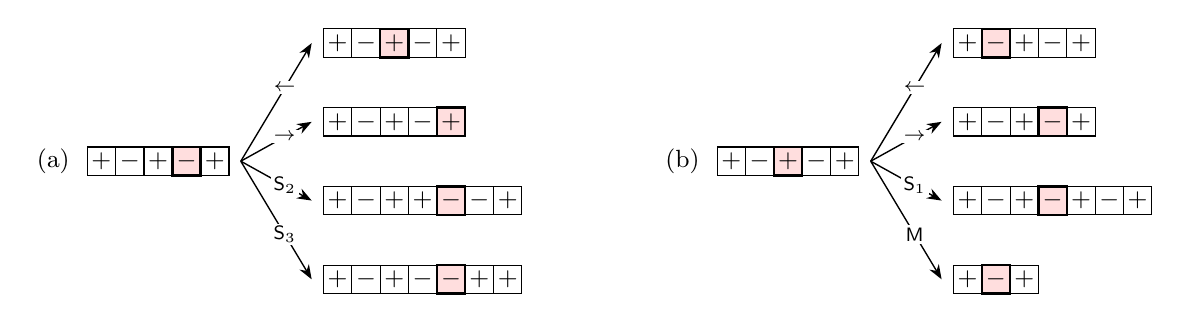
\begin{tikzpicture}[>=Stealth]
  % panel (a): head on -
  \tp{(0,0)}{+,-,+,-,+}{4}
  \node[font=\small,anchor=east] at (-0.1,0) {(a)};
  \tp{(3.0,1.5)}{+,-,+,-,+}{3}
  \tp{(3.0,0.5)}{+,-,+,-,+}{5}
  \tp{(3.0,-0.5)}{+,-,+,+,-,-,+}{5}
  \tp{(3.0,-1.5)}{+,-,+,-,-,+,+}{5}
  \foreach \yy/\lab in {1.5/{$\Lm$},0.5/{$\Rm$},-0.5/{$\Stwo$},-1.5/{$\Sthree$}} {
    \draw[->,line width=0.5pt] (1.95,0)--(2.85,\yy) node[pos=0.62,fill=white,inner sep=1pt,font=\scriptsize] {\lab};}
  % panel (b): head on +
  \begin{scope}[xshift=8.0cm]
  \tp{(0,0)}{+,-,+,-,+}{3}
  \node[font=\small,anchor=east] at (-0.1,0) {(b)};
  \tp{(3.0,1.5)}{+,-,+,-,+}{2}
  \tp{(3.0,0.5)}{+,-,+,-,+}{4}
  \tp{(3.0,-0.5)}{+,-,+,-,+,-,+}{4}
  \tp{(3.0,-1.5)}{+,-,+}{2}
  \foreach \yy/\lab in {1.5/{$\Lm$},0.5/{$\Rm$},-0.5/{$\Sone$},-1.5/{$\Mm$}} {
    \draw[->,line width=0.5pt] (1.95,0)--(2.85,\yy) node[pos=0.62,fill=white,inner sep=1pt,font=\scriptsize] {\lab};}
  \end{scope}
\end{tikzpicture}
\caption{The moves at two tapes. (a) The tape $+-+[-]+$ of Figure~\ref{fig:cut}, with the head on a $-$: two head
moves and two splits. (b) The tape $+-[+]-+$ reached after crossing $4$, with the head on a $+$: two head moves, one
split and the merge $-[+]-\mapsto[-]$, which returns to the root. The shaded box is the head.}
\label{fig:moves}
\end{figure}

A \emph{walk} is a sequence of tapes in which each tape is obtained from the previous one by a move; its length is
the number of moves. A \emph{closed walk} is a walk that starts and ends at the root.

\begin{theorem}[tape machine]\label{thm:tape}
For every $n\ge1$, reading the crossings $2,\ldots,2n-1$ of a meander as moves is a bijection between the meanders of
order $n$ and the walks of $2n-2$ moves of Table~\ref{tab:moves} that start at the root $+[-]+$ and end at the root.
\end{theorem}

\begin{proof}[Idea of the proof]
\emph{Labels.} Deleting crossing $2n$ turns the road into a path, and Lemma~\ref{lem:labels} gives labels that change
by $\pm1$ along arches and between neighbors along the river.

\emph{Stacks and differences.} At each cut the open arches form two stacks of labels, and the numbers
\eqref{eq:path} form a path with steps $\pm1$; its steps and the marked step are the tape. The tape recovers both
stacks.

\emph{One crossing, one move.} Revealing the next crossing pushes or pops each stack, and the case analysis above
shows that the possible updates are exactly the moves of Table~\ref{tab:moves}, that different updates give different
tapes, and that twin stack states lead to the same tapes. Hence a walk of tapes starting at the root lifts in exactly
one way to a walk of stack states, and it ends at the first stack state if and only if the tape walk ends at the
root (the root has head letter $-$, so its label is determined). The first crossing creates the root and the last
crossing closes the two remaining arches, so a meander of order $n$ gives a closed walk of $2n-2$ moves.

\emph{Back to a meander.} Conversely, replay a closed walk from the root, remembering at which crossing each arch was
opened. Every closing joins the current crossing to the most recently opened arch on its side, so the arches do not
cross; at the end one arch remains on each side and both are joined to a final crossing $2n$. The labels obey
\eqref{eq:arch} and the neighbor rule by construction, so by the converse half of Lemma~\ref{lem:labels} the arches
form one closed road. The two constructions undo each other.
\end{proof}

The same proof works on a strip: closed walks whose gap numbers stay in a fixed range of $K$ consecutive integers
count the meanders whose labels stay in the same range extended by one value at the top, a fixed band of $K+1$
integers. For example, gap numbers from $-1$ to $1$ correspond to labels from $-1$ to $2$. Strips are used for the
lower bound (Section~\ref{sec:flows}).

\paragraph{The excluded merge and the one-road property.}
The machine never closes a loop too early. Such a step would be a crossing that closes, on both sides, two arches
belonging to the same piece of road. No allowed move does this. Every tape reached from the root can be completed to a closed walk
(Lemma~\ref{lem:sweep} below), every closed walk gives a single road (the converse half of
Lemma~\ref{lem:labels}), and a loop closed early would survive in the completion as a second component. At a head
$-$ the machine has no merge at all: there the two innermost arches carry the same label, and the label of the new
crossing would have to be one more and one less than that label at once. The merge at $+[+]+$ is missing for a
different reason, label consistency: after it the arch below would force the next label down and the arch above would
force it up, so no continuation exists. The local rules know nothing about connectivity; it is the planar argument of
Lemma~\ref{lem:labels} that turns the label rules into the global condition that the road is one closed curve.
% Author's check, not in the sources (script written for this paper): over all histories of at most 11 moves, at every
% tape with head letter + the two innermost open arches belong to different pieces of road, including at + [+] +.
% UNVERIFIED as a general statement; not used anywhere.

\subsection{Worked examples}

\emph{Order $2$.} The root has four moves: $\Lm$, $\Rm$, $\Stwo$, $\Sthree$. After a split the head is on a $-$,
where no merge applies, so only the head moves can be undone in one more move. The closed walks of $2$ moves are
therefore $\Lm\Rm$ and $\Rm\Lm$:
\[ +[-]+ \xrightarrow{\ \Lm\ } [+]-+ \xrightarrow{\ \Rm\ } +[-]+, \qquad
   +[-]+ \xrightarrow{\ \Rm\ } +-[+] \xrightarrow{\ \Lm\ } +[-]+ . \]
The first gives the lower arches $1$--$2$, $3$--$4$ and the upper arches $1$--$4$, $2$--$3$; the second is its mirror
image. These are the $M_2=2$ meanders.

\emph{Order $3$.} The running example is the closed walk $\Rm\,\Sone\,\Lm\,\Mm$. Table~\ref{tab:example} follows it
crossing by crossing.

\begin{table}[htb]
\centering
\small
\setlength{\tabcolsep}{4pt}
\begin{tabular}{cclcccl}
\toprule
crossing & label & arches at this crossing & $\sigma$ & $\tau$ & tape after it & move \\
\midrule
$1$ & $0$ & opens lower $1$--$6$, upper $1$--$2$ & $(0)$ & $(0)$ & $+[-]+$ & (start)\\
$2$ & $-1$ & closes upper $1$--$2$, opens lower $2$--$5$ & $(0,-1)$ & $()$ & $+-[+]$ & $\Rm$\\
$3$ & $0$ & opens lower $3$--$4$, upper $3$--$6$ & $(0,-1,0)$ & $(0)$ & $+-+[-]+$ & $\Sone$\\
$4$ & $1$ & closes lower $3$--$4$, opens upper $4$--$5$ & $(0,-1)$ & $(0,1)$ & $+-[+]-+$ & $\Lm$\\
$5$ & $0$ & closes lower $2$--$5$ and upper $4$--$5$ & $(0)$ & $(0)$ & $+[-]+$ & $\Mm$\\
$6$ & & closes lower $1$--$6$ and upper $3$--$6$ & & & & (end)\\
\bottomrule
\end{tabular}
\caption{The running example as a walk of the tape machine. The merge at crossing $5$ is $-[+]-\mapsto[-]$.}
\label{tab:example}
\end{table}

The other seven meanders of order $3$ are the walks $\Lm\Rm\Lm\Rm$, $\Lm\Rm\Rm\Lm$, $\Rm\Lm\Lm\Rm$, $\Rm\Lm\Rm\Lm$,
$\Lm\,\Sone\,\Rm\,\Mm$, $\Stwo\,\Lm\,\Mm\,\Rm$ and $\Sthree\,\Rm\,\Mm\,\Lm$. Counting closed walks by computer gives
\[ 1,\ 2,\ 8,\ 42,\ 262,\ 1828,\ 13820,\ 110954,\ \ldots \]
for $n=1,2,3,\ldots$, the meander numbers; the counts were compared with the exact table up to $n=15$. A
correct count for small $n$ is a check of the implementation, not a proof; the proof is Theorem~\ref{thm:tape}.

\subsection{Basic facts}

Let $\cls$ be the class of tapes with at least three letters whose first and last letters are $+$ and whose letters
sum to $1$ (counting $+$ as $+1$ and $-$ as $-1$). The root is in $\cls$, and every move maps $\cls$ to itself: a split
replaces a letter by three with the same sum, a merge replaces three by one with the same sum, and neither changes an
end letter $+$ into $-$. A merge never acts on a tape of three letters, because the only such tape in $\cls$ is $+-+$,
whose middle letter is $-$.
Let $a$ and $b$ be the numbers of letters to the left and to the right of the head. The moves change $(a,b)$ by
\begin{equation}\label{eq:drift}
  \Lm:(-1,+1),\qquad \Rm:(+1,-1),\qquad \text{splits}:(+1,+1),\qquad \Mm:(-1,-1).
\end{equation}
So $a$ changes parity at every move, and a closed walk has an even number of moves.

\begin{lemma}[linear completion]\label{lem:sweep}
Every tape of $\cls$ with $N$ letters can be reached from the root in at most $3N$ moves, and the root can be reached
from it in at most $3N$ moves, through tapes with at most $N$ letters.
\end{lemma}

\begin{proof}
A merge deletes the head letter $+$ and one neighboring $-$, and leaves the other neighbor in place. A split read
backward deletes the head letter $-$ and one neighboring $+$. Put the head on the second letter and sweep to the right,
keeping the inner letters before the head all equal. When the head and the inner letter before it differ, delete this
pair, by a merge for the return and by a backward split for the build, after at most one head move; the head moves
back by at most two places. Otherwise move right. When the head reaches the last letter, all inner letters are equal
and sum to $-1$, so the tape is $+-+$. There are $(N-3)/2$ deletions; counting the moves gives at most $3N$. Read
backward, the build is a legal walk from the root, because head moves are reversible and a backward split read forward
is a split.
\end{proof}

Closed walks can be concatenated: one closed walk followed by another is again a closed walk. Write $c_t$ for the
number of closed walks of $t$ moves, so that $c_{2n-2}=M_n$. Then $c_tc_{t'}\le c_{t+t'}$, and since at most four moves
apply at any tape, $c_t\le 4^t$. By Fekete's lemma on supermultiplicative sequences
\begin{equation}\label{eq:fekete}
  \mu=\lim_{n\to\infty}c_{2n}^{1/n}=\sup_n c_{2n}^{1/n},\qquad\text{so}\qquad c_t\le\mu^{t/2}\ \text{for every even }t.
\end{equation}
This is also why squares appear in both bounds: one unit of $n$ is two moves.

% Section 3. Sources: 607_bounds_paper/paper.tex section 3 (weight inequality, four points, best weight, ledger);
% 641_tape_window_bounds/PROOF.md Lemma U; 607_bounds_paper/paper_word.tex section 3.1 (edge certificate);
% 1003_paired_path_consistency/PROOF.md section 1 (finite SOS theorem), section 4 (field is not a potential);
% 1251_referee_upper_12297/STATEMENT.md and FINAL.md section 2 (normalization); 1201_upper_structures/FINAL.md
% (edge-class inventory: Perron vectors give equality).
%%%%%%%%%%%%%%%%%%%%%%%%%%%%%%%%%%%%%%%%%%%%%%%%%%%%%%%%%%%%%%%%%%%%%%%%
\section{From weights to an upper bound}\label{sec:weights}
%%%%%%%%%%%%%%%%%%%%%%%%%%%%%%%%%%%%%%%%%%%%%%%%%%%%%%%%%%%%%%%%%%%%%%%%

A \emph{history} is a walk of the tape machine that starts at the root and may end anywhere. A \emph{successor} of a
tape is a tape one move later; a \emph{predecessor} is a tape one move earlier. By Theorem~\ref{thm:tape} and
\eqref{eq:fekete}, bounding $\mu$ from above means bounding the number of closed walks.

\subsection{One weight}

Let $W$ assign a positive number $W(T)$ to every tape $T$ of $\cls$, and suppose that for some $R$ and every tape $T$
of $\cls$,
\begin{equation}\label{eq:sub}
  \sum_{T'\ \text{successor of}\ T} W(T') \;\le\; R\,W(T).
\end{equation}
Intuitively, every tape has at most $R$ continuations, when continuations are counted by weight and not by number.

\begin{lemma}\label{lem:oneweight}
If \eqref{eq:sub} holds at every tape of $\cls$, then $M_n\le R^{2n-2}$ for every $n$, and $\mu\le R^2$.
\end{lemma}

\begin{proof}
Give each history the weight of its last tape. One more move replaces a history ending at $T$ by one history for each
successor of $T$, and by \eqref{eq:sub} their weights add up to at most $R\,W(T)$. So the histories of $t$ moves have
total weight at most $R^tW(\text{root})$. Those that end at the root weigh $W(\text{root})$ each, and all others have
positive weight, so at most $R^t$ histories of $t$ moves end at the root. Put $t=2n-2$ and use
Theorem~\ref{thm:tape}.
\end{proof}

Intuitively, the proof keeps a running total of the weights of all histories, and this total grows by at most a
factor $R$ per move. After four moves eight histories are back at the root, the eight meanders of order $3$; the
others are counted too, which makes the bound loose but not wrong. Four points of the argument are easy to get
wrong~\cite{BoundsPaper}. The inequality is about the \emph{sum}: a single successor may weigh more than the present
tape. A history carries \emph{one} weight, that of its current tape; the factors $W(T')/W(T)$ along a history
telescope. Histories that do not return to the root are \emph{kept}, with positive weight. And weights are \emph{not
probabilities}: their only job is to satisfy \eqref{eq:sub}.

With all weights equal, \eqref{eq:sub} holds with $R=4$, the largest number of moves at a tape, and gives the trivial
bound $\mu\le16$. Unequal weights help because tapes differ in how many continuations they have; for example a tape
with the head on a $-$ has no merge, and a tape with the head at an end has one head move fewer. The ideal weight would
be the number of ways to return to the root in a given number of moves, which is the original counting problem. The
weights used below are tractable stand-ins, and they are valid only because the inequality is checked everywhere. In
matrix language, \eqref{eq:sub} says $AW\le RW$ for the $0/1$ matrix $A$ of the moves, and
Lemma~\ref{lem:oneweight} is the easy half of the Collatz--Wielandt characterization of the Perron root, the largest
eigenvalue of a nonnegative matrix~\cite{Seneta}.


\subsection{Two weights and reciprocal edge factors}

The certificate of Section~\ref{sec:upper} uses a sharper test. It looks at each tape both forward, along its moves,
and backward, along the moves that lead into it, and it lets each move carry a factor that its reverse pays back.
Intuitively, a move may borrow weight as long as the reverse move returns it.

Let $X$ be a finite set of tapes and $A$ its $0/1$ matrix of moves, with rows and columns indexed by the tapes:
$A_{TT'}=1$ if a move goes from $T$ to $T'$, both in $X$. Choose positive weights $W(T)$ and $Z(T)$ on $X$. Call
$\{T,T'\}$ an \emph{edge} if a move goes from $T$ to $T'$ or from $T'$ to $T$, and choose for every edge a positive
factor $\theta_{TT'}$ with
\begin{equation}\label{eq:recip}
  \theta_{T'T}=1/\theta_{TT'}.
\end{equation}
The \emph{row value} of tape $T$ is
\begin{equation}\label{eq:row}
  \phi_T \;=\; \frac12\sum_{T':\ T\to T'}\theta_{TT'}\,\frac{W(T')}{W(T)}\;+\;\frac12\sum_{T':\ T'\to T}\theta_{TT'}\,\frac{Z(T')}{Z(T)}.
\end{equation}
The first sum runs over successors, the second over predecessors. In both, the factor is the one oriented from the
present tape $T$ toward its neighbor $T'$, not the one in the direction of the move. Confusing the two orientations
would invalidate the certificate.

\begin{lemma}[paired rows]\label{lem:paired}
If $\phi_T\le R$ for every $T\in X$, then the spectral radius of $A$ is at most $R$.
\end{lemma}

\begin{proof}
Put
\[ B_{TT'}=A_{TT'}\sqrt{\frac{Z(T)\,W(T')}{W(T)\,Z(T')}},\qquad
   \vartheta_{TT'}=\theta_{TT'}\sqrt{\frac{W(T')\,Z(T')}{W(T)\,Z(T)}} . \]
The matrix $B$ is obtained from $A$ by conjugating with a positive diagonal matrix, so it has the same spectral
radius $\rho(A)$. Let $\widehat B=\frac12(B+B^{\mathsf T})$ be its symmetric part. Then
$\vartheta_{T'T}=1/\vartheta_{TT'}$, and a short computation gives $\widehat B_{TT'}\vartheta_{TT'}=\frac12\bigl(A_{TT'}W(T')/W(T)+A_{T'T}Z(T')/Z(T)\bigr)\theta_{TT'}$,
so that $\phi_T=\sum_{T'}\widehat B_{TT'}\vartheta_{TT'}$. For every edge and every real vector $v$,
$2v_Tv_{T'}\le \vartheta_{TT'}v_T^2+\vartheta_{T'T}v_{T'}^2$, since the difference is
$\bigl(\sqrt{\vartheta_{TT'}}\,v_T-v_{T'}/\sqrt{\vartheta_{TT'}}\,\bigr)^2$. Summing over the edges with the weights
$\widehat B_{TT'}\ge0$ gives
\[ v^{\mathsf T}\widehat Bv\;\le\;\sum_T\phi_Tv_T^2\;\le\;R\,\lvert v\rvert^2 . \]
A move always changes the tape, so $A$ has no diagonal entries. The matrix $B\ge0$ has a nonnegative eigenvector $v$
for its spectral radius $\rho(A)$, and for it $v^{\mathsf T}\widehat Bv=v^{\mathsf T}Bv=\rho(A)\lvert v\rvert^2$. Hence
$\rho(A)\le R$.
\end{proof}

\begin{corollary}\label{cor:paired}
If $\phi_T\le R$ holds for every finite set $X$ of tapes of $\cls$ and every $T\in X$, then $M_n\le R^{2n-2}$ for
every $n$, and $\mu\le R^2$.
\end{corollary}

\begin{proof}
Fix $n$ and $t=2n-2$, and let $X$ be the tapes of $\cls$ with at most $t+3$ letters; every closed walk of $t$ moves
stays in $X$, and so does every concatenation of such walks. So $(A^{\ell t})_{\text{root},\text{root}}\ge
M_n^{\,\ell}$ for every $\ell\ge1$. Taking $\ell t$-th roots and letting $\ell\to\infty$ gives
$M_n^{1/t}\le\rho(A)\le R$.
\end{proof}

The argument uses finite matrices only; it never assumes that a change of weights is valid on the infinite set of
all tapes.
Restricting to $X$ only deletes positive terms from \eqref{eq:row}, so in practice one checks the row values with all
neighbors present.

\paragraph{Why two weights and edge factors help.}
Lemma~\ref{lem:oneweight} looks at successors only. Averaging the forward and the backward view lets the slack of
one direction (the amount by which its sum falls below $R$) pay for the other. The edge factors add a freedom that no
weight on tapes has.
The ratios $W(T')/W(T)$ of a single weight multiply to one around every closed cycle of moves; reciprocal edge factors need
only invert along the \emph{same} edge, so around a cycle they can multiply to anything. They are parameters of the
inequality, not move probabilities. On a finite set of tapes, taking for $W$ and $Z$ the right and left Perron
vectors of $A$ (its eigenvectors for the spectral radius) and all factors equal to one makes every row value equal to
the spectral radius. So the Perron vectors are the ideal choice, and improving a certificate means describing them
better by features that can be read near the head.

It is natural to take $Z$ to be $W$ of the complemented tape $\cpl T$, in which every letter is changed. Reversing a
move and complementing the tape gives a forward move: the reverse of the split $[+]\mapsto+[-]+$ is
$+[-]+\mapsto[+]$, whose complement $-[+]-\mapsto[-]$ is a merge, and the same holds for the other splits and merges;
head moves are their own reverses. So the predecessors of $T$ are the complements of the successors of $\cpl T$, and
the backward sum of \eqref{eq:row} is a forward sum for the complemented tape. The missing merge at $+[+]+$ has no
edge in either direction.

% Section 4. Sources: 641_tape_window_bounds/PROOF.md section 2 (weight family, Lemmas 1-2, padding);
% 1003_paired_path_consistency/PROOF.md sections 2-3 (head factors, cut convention, locality);
% 1007_edit_edge_1230/PROOF.md (edit factors, triples, symmetries); 1201_upper_structures/PROOF.md (k = r+1 lemma)
% and FINAL.md (certificate, tables of matched tests, run times); 1201 runs/r9_run2_verify.json (exact R, argmax);
% 1251_referee_upper_12297/FINAL.md (sharpness of locality, independent replay); 607_bounds_paper/paper_word.tex
% section 3 (symmetries, convexity); web/src/meandric/TapeMachineWriteup.tsx (single-weight tape certificates and the
% value 15.89 for the table alone at radius 6).
%%%%%%%%%%%%%%%%%%%%%%%%%%%%%%%%%%%%%%%%%%%%%%%%%%%%%%%%%%%%%%%%%%%%%%%%
\section{The upper-bound certificate}\label{sec:upper}
%%%%%%%%%%%%%%%%%%%%%%%%%%%%%%%%%%%%%%%%%%%%%%%%%%%%%%%%%%%%%%%%%%%%%%%%

Corollary~\ref{cor:paired} needs the row inequality $\phi_T\le R$ at every tape $T$ of $\cls$, and there are
infinitely many. This section describes weights and factors whose row values depend only on the letters near the
head, so that a finite list of cases suffices, and then the certificate that proves the upper bound of
Theorem~\ref{thm:main}.

\subsection{The weights}

Fix a whole number $r$, the \emph{radius}. To evaluate weights, pad each end of a tape with $r+1$ extra letters $-$,
so that the letters near the head are defined even when the head is close to an end; the padding is not part of the
machine. The \emph{window} of a tape is the word of the $2r+1$ letters centered on the head. The \emph{left side} is
the word of the letters left of the head, read from the far end toward the head; the \emph{right side} is the word of
the letters right of the head, also read from the far end toward the head. A \emph{$k$-gram} of a word is a block of
$k$ consecutive letters. Fix a \emph{gram length} $k\ge1$ and positive tables $U$ on windows and $V$ on words of $k$
letters, and set
\begin{equation}\label{eq:W}
  W(T)\;=\;U(\text{window of }T)\cdot\prod_{\gamma}V(\gamma),
\end{equation}
where $\gamma$ runs over the $k$-grams of the left side and of the right side. Let $Z(T)=W(\cpl T)$, where $\cpl T$
complements every letter, padding included. Intuitively, the table $U$ judges the tape near the head, where the next
move acts, and the factors $V$ judge the whole tape by its short patterns.

\subsection{The edge factors}

There are two kinds of edges. A \emph{head edge} joins a tape to the same word with the head moved by one letter. Fix
$q\ge1$ and a positive table $E$ on words of $2q$ letters. A move of the head one letter to the right reads the
\emph{boundary word}, the $2q$ letters centered on the boundary between the old and the new head position, and has
the factor $E$ of that word. The reverse move reads the same boundary word and has the factor $1/E$.

An \emph{edit edge} joins a short tape to a long tape in which the head letter is replaced by three letters, with the
head on the middle one. For a short letter $-$ the triples are $--+$, $-+-$, $+--$; for a short letter $+$ they are
$-++$, $+-+$, $++-$. Three of the six are splits ($+-+$, $+--$, $--+$) and the other three are reverses of merges.
The triple $+++$ has no edge, because the merge at $+[+]+$ does not exist. Fix $d\ge1$ and a positive table $G$ on
pairs (window of radius $d$ around the head of the short tape, triple). The factor is $G$ from short to long and $1/G$
from long to short. So every edge and its reverse have reciprocal factors, as \eqref{eq:recip} requires.

The tables used have symmetries: $U$ is unchanged when its window is reversed; $E$ is unchanged when its boundary
word is complemented and is inverted when that word is reversed; and $G$ is unchanged when both the window and the
triple are complemented or both are reversed. The symmetries reduce storage and search; the proof does not need them.

\subsection{Reduction to finitely many cases}

A \emph{formal row} is a word of $2r+3$ letters with the head on the middle letter. Its row value is \eqref{eq:row}
computed on the formal row itself, as a stand-alone word with all its moves and all its predecessors, the weights and
factors being read from its letters.

\begin{lemma}[locality]\label{lem:local}
Suppose $k\le r+1$, $q\le r+1$ and $d\le r$. For every move, the ratios $W(T')/W(T)$ and $Z(T')/Z(T)$ and the edge
factor depend only on the letters of $T$ at distance at most $r+1$ from the head.
\end{lemma}

\begin{proof}
The $k$-grams away from the head appear in both weights and cancel. A head move to the left removes the last $k$-gram
of the left side, which ends next to the head, and adds one $k$-gram to the right side, which ends at the old head
letter: the letters used lie within distance $k$ on the left and $k-1$ on the right. A head move to the right is the
mirror image. A split adds one letter at the inner end of each side, so its new grams use letters within distance
$k-1$. A merge removes the inner letter of each side, and the lost grams reach distance $k$. The window of radius $r$
around a head that moved by one letter lies within distance $r+1$, the boundary word has $q\le r+1$ letters on each
side of the boundary, and the short window of an edit edge, of radius $d$ around the short head, reaches at most $d+1\le r+1$ letters
from the head of the long tape. Complementing every letter gives the same statements for $Z$.
\end{proof}

The conditions cannot be relaxed by one: with $k=r+2$, or $q=r+2$, or $d=r+1$, a test with random tables finds tapes
where locality fails. Earlier certificates of the project used $k\le r$; that was a restriction of the programs, not
of the theory.

\begin{proposition}[finitely many cases suffice]\label{prop:rows}
Suppose the conditions of Lemma~\ref{lem:local} hold and every one of the $2^{2r+3}$ formal rows has row value at
most $R$. Then $\phi_T\le R$ for every tape $T$ in every finite set of tapes of $\cls$, and so $M_n\le R^{2n-2}$ and
$\mu\le R^2$.
\end{proposition}

\begin{proof}[Idea of the proof]
Take a tape, padded. Its $2r+3$ letters around the head form a formal row. By Lemma~\ref{lem:local}, every move and
every predecessor of the tape has the same ratio and the same factor as the corresponding term of the formal row.
The formal row may have more terms, for example a head move into the padding or a move leaving the finite set, but
all terms are positive. So the row value of the tape is at most that of its formal row. Apply
Corollary~\ref{cor:paired}.
\end{proof}

Here no case is a worst case over letters that the formal row cannot see: a formal row determines every ratio
exactly, because no move acts away from the head. This is the main difference from the window method on bracket
words~\cite{BoundsPaper}, where a move can involve a letter far from the window.

\subsection{The certificate}

Table~\ref{tab:upper} lists the certificate behind Theorem~\ref{thm:main}. All $2{,}097{,}152$ formal rows were
evaluated in exact rational arithmetic, with every move made literally on the word, and the largest row value is the
number $R_+$ stored as an exact rational in the verification report, alongside the weight certificate. Then
\[ \mu\;\le\;R_+^2\;=\;12.29693385352921289818\ldots\;<\;12.296933854 . \]

\begin{table}[htb]
\centering
\begin{tabular}{ll}
\toprule
radius $r$ (window of $U$) & $9$ ($19$ letters) \\
gram length $k$ & $10$ \\
boundary word of a head edge & $2q=20$ letters \\
edit window & radius $d=9$ around the short head \\
formal rows & $2^{21}=2{,}097{,}152$ \\
free parameters (after the symmetries) & $918{,}784$ \\
largest row value $R_+$ & $3.50669842637333\ldots$ (exact fraction) \\
bound $R_+^2$ & $12.29693385352921289818\ldots$ \\
exact check, one thread & $255$~s; independent checker $292$~s \\
\bottomrule
\end{tabular}
\caption{The upper-bound certificate.}
\label{tab:upper}
\end{table}

\paragraph{How the tables were found.}
Each row value is a sum of products of table entries with positive coefficients. In the logarithms of the entries,
each term is the exponential of a linear function, so the largest row value is a convex function of these logarithms.
The search minimized a smooth version of the largest row value (a log-sum-exp with a large parameter) by a
quasi-Newton method (L-BFGS). A radius-$8$ certificate ($12.299756359$) was rewritten exactly in the larger family of
radius $9$ and gram length $10$, as a starting point. Two runs of about $2{,}500$ and $2{,}200$ seconds on one thread
then brought the bound to $12.297636863$ and to $12.296933854$. None of this is part of the proof, which consists of
the stored tables and the exact check of all rows.

\paragraph{The contribution of each ingredient.}
Table~\ref{tab:ingredients} compares the ingredients at small radius, where the optimum can be found reliably; its
values are floating-point optima, not certified bounds. At radius $4$ the edit factors lower $R^2$ by $0.034$, about
three quarters of the gain of one step of radius ($0.046$), with fewer than half as many free parameters ($920$
against $2{,}080$ for head factors alone at radius $5$). The longer gram length is a real but small gain. The $k$-gram factors do most of the work overall: for a single
weight, the table $U$ alone gives only $15.89$ at radius $6$, and single weights with $8$-gram factors needed radius
$12$ to certify $\mu\le12.3889$.

\begin{table}[htb]
\centering
\begin{tabular}{lccc}
\toprule
radius & head factors only & head and edit factors & same, with gram length $r+1$ \\
\midrule
$4$ & $12.40026$ & $12.36583$ & $12.36392$\\
$5$ & $12.35452$ & $12.33585$ & $12.33555$\\
\bottomrule
\end{tabular}
\caption{Best values of $R^2$ found at small radius for three parts of the family (floating point, not bounds).}
\label{tab:ingredients}
\end{table}
% Source: 1201 FINAL, matched small-radius tests, rows a = 5 (r = 4) and a = 6 (r = 5); (rU,k,q,d) = (4,4,5,0),
% (4,4,5,4), (4,5,5,4) and (5,5,6,0), (5,5,6,5), (5,6,6,5). Value 15.89 and 12.3889: web TapeMachineWriteup.tsx.

% Section 5. Sources: 641_tape_window_bounds/PROOF.md Lemma L; 607_bounds_paper/paper.tex section 5 (finite region);
% 805_entropy_certificates/PROOF.md section 1 (Theorem F, proof steps 1-4, remarks); 808_referee_flow_bound/FINAL.md;
% 1252_referee_lower_theory/PROOF.md sections 0-2 (strip, memory m, Proposition A, Theorem F', remarks) and FINAL.md
% section 3 (tests on strips); 607_bounds_paper/paper_word.tex section 4 (exposition).
%%%%%%%%%%%%%%%%%%%%%%%%%%%%%%%%%%%%%%%%%%%%%%%%%%%%%%%%%%%%%%%%%%%%%%%%
\section{From flows to a lower bound}\label{sec:flows}
%%%%%%%%%%%%%%%%%%%%%%%%%%%%%%%%%%%%%%%%%%%%%%%%%%%%%%%%%%%%%%%%%%%%%%%%

For a lower bound we must exhibit many closed walks. An upper bound may count too much; a lower bound may count too
little. This section first recalls the weight inequality with the direction reversed, which gives lower bounds, and
then describes the entropy method used for the lower bound of Theorem~\ref{thm:main}.

\subsection{Counting inside a finite region}

\begin{lemma}\label{lem:region}
Let $\psi\ge0$ be a weight on the tapes of $\cls$ that is zero on every tape with more than $N$ letters and has
$\psi(\text{root})>0$. Suppose that $\sum_{T'}\psi(T')\ge R\,\psi(T)$ at every tape $T$ with $\psi(T)>0$, the sum running
over the successors. Then $\mu\ge R^2$.
\end{lemma}

\begin{proof}
Follow all histories from the root and delete a history when it reaches a tape of weight zero. Each move multiplies
the total weight of the survivors by at least $R$, so after $t$ moves at least $R^t\psi(\text{root})/\max\psi$
histories survive. Each survivor ends at a tape with at most $N$ letters and can be closed by Lemma~\ref{lem:sweep} in a
bounded number of moves, and different survivors with the same end tape give different closed walks. The closed walks
have boundedly many different lengths, so one length gets a fixed fraction of them. Neither the extra moves nor the
fraction changes the growth rate.
\end{proof}

The earlier lower bound $12.0535$~\cite{BoundsPaper} came from this lemma on the bracket encoding and needed $1.26$
billion table entries: the region must be large and the weight must fade toward its boundary. The entropy method
works on infinite tapes and has no such boundary.

\subsection{Counting by entropy}

Choose a random rule for the next move that looks only at the letters near the head. Intuitively, if the rule makes
on average $e^h$ equally likely choices per move, then it produces about $e^{ht}$ different histories of $t$ moves. If
the rule is stationary, so that the tape seen from the head looks statistically the same at all times, and if on
average it neither lengthens the tape nor moves the head to one side, then a typical history stays within a short
stretch of tape, and Lemma~\ref{lem:sweep} closes it at small cost. Then $c_t$ is at least about $e^{ht}$, and
\eqref{eq:fekete} gives $\mu\ge e^{2h}$. The work is to make such a rule exactly stationary on infinite tapes while
writing it with finitely many numbers. Theorem~F below makes this precise.

\subsection{Stationary flows}

\emph{The strip.} Fix $K\ge2$, or $K=\infty$. Read a tape as a path of heights: a starting height, then one step
up or down per letter. For a tape reached from the root the heights are the gap numbers \eqref{eq:path} plus
$\lfloor K/2\rfloor$; moves never change the starting height. A tape lies in the \emph{strip of height $K$} if all
heights lie in $\{0,\ldots,K-1\}$. On the strip, a split is allowed only if the new path stays in the strip; head
moves and merges never leave it. Closed walks from the root on a strip count the meanders whose labels stay in the
fixed band $-\lfloor K/2\rfloor\le g\le K-\lfloor K/2\rfloor$ of $K+1$ values (Section~\ref{sec:tape}); for even
$K$ this is $-K/2\le g\le K/2$. Their growth rate $\Lambda_K$ is at most $\mu$.

\emph{The reference law.} An infinite tape is a two-sided infinite path of heights in the strip with a head at one
letter. The \emph{reference law} $\beta$ is a stationary Markov chain on such paths with \emph{memory} $m$: the
probability of the next step depends on the current height and the last $m$ steps. We assume that every path of $m+2$
heights in the strip has positive probability and that the chain is irreducible. For a finite word $w$ with given
heights, $\beta(w)$ is its probability. The reference law is a fixed background; it describes the tape far from the
head.

\emph{Windows and flows.} Fix a radius $r$. A \emph{window} $w$ is the word of the $2r+1$ letters centered on the head,
together with its heights. A \emph{flow} is a family of numbers $J(w,\xi)\ge0$, the \emph{flow values}, one for each
window $w$ and each move $\xi$ that applies at $w$ in the strip, with total $1$. Intuitively, $J(w,\xi)$ is the
probability that the window is $w$ and the next move is $\xi$. Put
\[ \nu(w)=\sum_\xi J(w,\xi),\qquad p(\xi\mid w)=J(w,\xi)/\nu(w). \]
The flow defines a random infinite tape and a random move: the window has law $\nu$; given the window, the letters
beyond it continue as the chain $\beta$, independently on the two sides, from the $m$ letters at each end of the
window; then the move $\xi$ is chosen with probability $p(\xi\mid w)$. Intuitively, the window is chosen by the flow
and the far tape by the reference law.

\emph{The conditions.}
\begin{itemize}
\item[(S)] \emph{Stationarity.} For every word $Y$ of $2r+3$ letters, with heights, let $Y^\circ$ be its middle
$2r+1$ letters. The probability that after the move the $2r+3$ letters around the head read $Y$ equals the probability
that they read $Y$ now:
\[ \sum_{w,\xi}J(w,\xi)\,\beta_{w,\xi}(Y) \;=\; \nu(Y^\circ)\,\frac{\beta(Y)}{\beta(Y^\circ)}, \]
where $\beta_{w,\xi}(Y)$ is the conditional probability, given the window $w$ and the reference law outside it, that
the move $\xi$ produces a tape whose $2r+3$ central letters are $Y$. We call these the \emph{balance equations}.
\item[(D)] \emph{Zero drift.} $\sum J(w,\xi)\,\Delta a(\xi)=\sum J(w,\xi)\,\Delta b(\xi)=0$, with the changes
$\Delta a,\Delta b$ of the side lengths from \eqref{eq:drift}. Intuitively, on average the tape does not grow and the
head does not travel.
\item[(P)] \emph{Positivity.} $J(w,\Lm)>0$ for every window $w$. It is used in Step~2 below to prove
ergodicity.
\end{itemize}
For a fixed reference law these are finitely many linear conditions on $J$. The following theorem, which we call
Theorem~F (for flow), turns them into a lower bound.

\begin{theoremF}
Let $r\ge m$, and let $J$ be a flow satisfying (S), (D) and (P). Then
\[ \mu\;\ge\;e^{2h},\qquad h\;=\;\sum_{w,\xi}J(w,\xi)\,\log\frac{\nu(w)}{J(w,\xi)} , \]
where terms with $J(w,\xi)=0$ are left out. In particular, if $h\ge\log R$ then $\mu\ge R^2$.
\end{theoremF}

The number $h$ is the entropy of the next move given the window, averaged over the stationary process: the
uncertainty of one move.

\subsection{Proof of Theorem F, in outline}

\emph{Step 1: the balance equations give stationarity of the whole tape.} Let the infinite tape have the law of the flow,
and make one move. A move changes only the head letter and its neighbors. Given the $2r+3$ letters around the new
head, the letters beyond them are again continuations of the chain from the $m$ letters at each end: for a head move
they are the old letters, for a split the old ends survive because $r\ge m$, and for a merge the two letters newly
brought into view are fresh chain letters. So the law of the new infinite tape is determined by the law of its $2r+3$
central letters, and (S) says that this law is the old one. The process is stationary. The radius condition $r\ge m$
is needed: in tests on small strips that compare the ranks of the linear systems, the balance equations with
$r=m-1$ do not imply those at larger radius, while with $r\ge m$ they do.

\emph{Step 2: the stationary process is ergodic.} By (P) the law of the flow has a positive density with respect to
$\beta$, so the two laws have the same null sets. Let $f$ be a bounded harmonic function, that is,
$\mathbb{E}[f(\omega_1)\mid\omega_0]=f(\omega_0)$ for the process $\omega_0,\omega_1,\ldots$ of infinite tapes. By
stationarity and harmonicity,
$\mathbb{E}\bigl(f(\omega_1)-f(\omega_0)\bigr)^2=2\mathbb{E}f(\omega_0)^2-2\mathbb{E}f(\omega_0)f(\omega_1)=0$, so
$f$ is unchanged by every move of positive probability, in particular by the move $\Lm$, which is a shift of the
infinite tape. The shift is ergodic for the irreducible chain $\beta$ (its period two does not matter), so $f$ is
constant. A stationary Markov process whose bounded harmonic functions are constant is ergodic.

\emph{Step 3: counting.} Write $t$ for the number of moves. Let $\Delta^a_i$ and $\Delta^b_i$ be the total changes
of the side lengths after $i$ moves, and $I_t$ the sum of $-\log p(\xi_i\mid w_{i-1})$ over the first $t$ moves. By the
ergodic theorem and (D), $\Delta^a_i/t$ and $\Delta^b_i/t$ tend to zero uniformly in $i\le t$, and $I_t/t$ tends to
$h$. Fix $\varepsilon>0$. For large $t$, with probability at least $1/2$, $|\Delta^a_i|+|\Delta^b_i|\le\varepsilon t$
for all $i\le t$ and $I_t\ge t(h-\varepsilon)$. From some fixed infinite tape this happens with conditional
probability at least $1/2$, and each move sequence in the event has probability at most $e^{-t(h-\varepsilon)}$, so
there are at least $\frac12e^{t(h-\varepsilon)}$ of them. Cut out the letters within distance
$\lceil\varepsilon t\rceil+r+2$ of the head. All these move sequences run on this finite piece, because the head never
comes within two letters of its ends. Pad the piece to a tape of $\cls$, build it from the root and return to the root
afterwards by Lemma~\ref{lem:sweep}; both cost $O(\varepsilon t)+O(1)$ moves, in the \emph{unrestricted} machine
(without the strip). Different move sequences give different closed walks, with lengths between $t$ and
$t+O(\varepsilon t)+O(1)$, so for one length $t'$ in this range $c_{t'}\ge e^{t(h-\varepsilon)}/\mathrm{poly}(t)$. With
$c_{t'}\le\mu^{t'/2}$ from \eqref{eq:fekete}, letting $t\to\infty$ and then $\varepsilon\to0$ gives
$h\le\frac12\log\mu$.\qed

\subsection{Remarks}

Only the middle part of the closed walks is confined to the strip; the counted walks are walks of the unrestricted
machine. So the bound concerns all meanders, but it can never exceed $\Lambda_K$. For a fixed reference law the
conditions are linear in $J$ and $h$ is concave in $J$. A flow is \emph{exactly feasible} if it satisfies (S), (D)
and (P) exactly, not up to rounding; every exactly feasible flow, optimal or not, gives a bound.

The method was tested where the answer is known. On the strip of three levels the growth rate
$\Lambda_3=10.4245356612\ldots$ is known exactly. The method reproduces it at radius $1$, $2$ and $3$, and to
$15$ digits with a memory-three reference law, and in no test does it exceed it. Without the drift condition
(D) the same computation gives $10.883$, above the true value. So (D) is essential, and the test is able to detect a
wrong method. Theorem~F was proved in the project for a reference law of memory two that looks at the letters only,
with no strip, and later written out for strips and for laws of any memory $m$ with $r\ge m$; both forms were read
independently (Appendix~\ref{app:where}).

% Section 6. Sources: 1228_combined_lower/FINAL.md (result, stages, increments, verifier); 1253_referee_lower_computation
% /FINAL.md (stage values, counts, law parameters, number of directions, parent counts); 1252_referee_lower_theory/PROOF.md
% sections 3-5 (Propositions B, C, D) and FINAL.md (law hypotheses H1-H3 exact, 154 five-paths);
% 1008_lower_122/PROOF.md (head cycles, four-move edit cycles, entropy enclosure); 1019_overnight_structural/
% MEMORY_THREE_EXTENSION.txt, SIGNED_PARENT_CERTIFICATE_ARGUMENT.txt, SPARSE_CONTEXT_REFINEMENT_ARGUMENT.txt;
% 607_bounds_paper/paper_word.tex section 5 (cycle example, figure); 1203_ceiling_ladder/FINAL.md section 1 (strip,
% kappa); ledger/STATE.md row "mu lower"; ledger/facts.json muLower.
%%%%%%%%%%%%%%%%%%%%%%%%%%%%%%%%%%%%%%%%%%%%%%%%%%%%%%%%%%%%%%%%%%%%%%%%
\section{The lower-bound certificate}\label{sec:lower}
%%%%%%%%%%%%%%%%%%%%%%%%%%%%%%%%%%%%%%%%%%%%%%%%%%%%%%%%%%%%%%%%%%%%%%%%

A certificate for Theorem~F is a reference law and an exactly feasible flow. Here we ask for a little more than (P):
the balance equations (S) and the drift equations (D) hold exactly, not up to rounding, and every flow value is
positive. At the radii we need, solving (S) exactly is too expensive. The certificate is therefore built from pieces
that are feasible by construction, and only positivity and the entropy are left to compute.

\subsection{The strip and the reference law}

The strip has height $K=12$. The reference law $\beta$ has memory three and is built in three layers. The first is a nearest-neighbor
law on the twelve heights; its probability of stepping up at heights $0,1,\ldots,11$ is
\[ 1,\ \tfrac{97}{100},\ \tfrac{99}{100},\ \tfrac{47}{50},\ \tfrac{171}{200},\ \tfrac{69}{100},\
   \tfrac{31}{100},\ \tfrac{29}{200},\ \tfrac{3}{50},\ \tfrac{1}{100},\ \tfrac{3}{100},\ 0, \]
symmetric under reflection of the strip. In the second layer, after a step up the odds of stepping up again are
multiplied by $\kappa=4/5$, and after a step down by $1/\kappa$, so the path changes direction a little more often.
In the third layer, each path of four heights gains probability if its first and last steps point in opposite
directions and loses it if they point the same way, by $\eta=3/16$ times the smallest probability among the paths
with the same middle heights up to reversal and reflection; then the same is done for paths of five heights, with
$\zeta=1/8$. Neither change alters the probabilities of shorter paths; each lets the next step depend on one more
earlier step. All hypotheses of Theorem~F on the law were checked in exact rational
arithmetic: the $154$ paths of $m+2=5$ heights in the strip have positive probability, the law is stationary, its
marginals are consistent, and the chain is irreducible.
% Law layers checked in the code: kappa in 914 edge_model.py (odds u_b/(1-u_b) * kappa^(b-a)), see 1203 PROOF
% section 1; eta in 1019 memory_two.py (quartet a,b,c,d with b,c interior: + eta * group minimum * sign, sign +1 when
% the first and last steps are opposite; triple marginals kept); zeta in 1019 memory_three.py (same on quintets with
% b,d interior; quartet marginals kept). Parameters as stored in the parent: 1253 FINAL item 4.

\subsection{Constructions that stay feasible}

The certificate combines four constructions. A \emph{direction} is a signed change of the flow values that keeps the
balance equations (S) and the drift equations (D) exactly; adding any multiple of a direction to an exactly feasible
flow leaves (S) and (D) exact, and only positivity has to be checked again.

\emph{A signed parent at a small radius.} At radius $6$ the system (S) and (D) was solved exactly in rational numbers.
The solution, the \emph{parent}, has $226{,}079$ flow values and satisfies all $220{,}110$ balance equations and both
drift equations; $7{,}708$ of its flow values are negative. A parent with negative values is allowed, because the
equations are linear and positivity is needed only for the final flow.

\emph{Lifting.} A nonnegative flow at radius $6$, after normalization, defines a law of the infinite tape, and the same law can
be read through windows of any larger radius. For the signed parent, the lift is defined by the same linear formula. The lifted flow value of a larger window is the old flow value of its central window times the
conditional reference probability of the extra letters; so the \emph{density} $J/\beta$, the flow divided by the
reference probability of the window, does not change. Lifting preserves (S), (D), and the total mass (the sum of all flow values). For a nonnegative flow it also
preserves the entropy after normalization; no entropy is assigned to the signed intermediate parent.

\emph{Closed walks.} The main source of directions is closed walks. Take a short tape $T_0$, the \emph{anchor}, and a
walk of moves that starts and ends at $T_0$. Suppose that no tape on the walk changes the starting height, the first
three letters, the last three letters, or the letter sum. Then the far tape beyond these \emph{protected ends} has the
same conditional law at every step. Fix a signed number $z$. For each move of the walk, from a tape $T$, add
$z\,\beta(T_0)/\beta(T)$ to the density $J/\beta$ of that move at every window whose central letters, with their
heights, spell $T$; that is, the flow value $J(w,\xi)$ grows by $z\,\beta(T_0)\beta(w)/\beta(T)$. If the walk makes the
same move from the same tape twice, the two amounts add. Each edge of the walk then carries the same
flow $z\,\beta(T_0)$ times the same law of the far tape, so at every tape the added inflow equals the added outflow:
the balance equations hold exactly, for every $z$. The drift vanishes because the walk is closed. The simplest walks
are the \emph{head cycles} $\Rm\Lm$, a step of the head and back. Next come four-move \emph{edit cycles}, which use a
split and a merge, such as $\Stwo\,\Lm\,\Mm\,\Rm$ from $+[-]+$ (Figure~\ref{fig:cycle}): split, step aside, merge, and
step back. Read from the root, this cycle is one of the eight meanders of order $3$; in the certificate the same
pattern runs inside longer tapes, whose protected ends it does not touch. The certificate also uses walks of six and
eight moves.

Protection matters. In tests on small strips, protecting only two letters at each end, or replacing the factor
$\beta(T_0)/\beta(T)$ by a constant, makes some random cycles violate the balance equations, and the tests detect it.

\begin{figure}[htb]
\centering
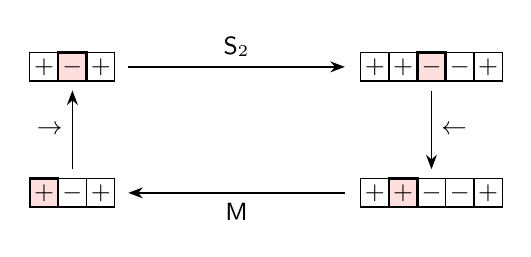
\begin{tikzpicture}[>=Stealth]
  \tp{(0,0)}{+,-,+}{2}
  \tp{(4.2,0)}{+,+,-,-,+}{3}
  \tp{(4.2,-1.6)}{+,+,-,-,+}{2}
  \tp{(0,-1.6)}{+,-,+}{1}
  \draw[->,line width=0.5pt] (1.25,0)--(4.0,0) node[midway,above,font=\small] {$\Stwo$};
  \draw[->,line width=0.5pt] (5.1,-0.3)--(5.1,-1.3) node[midway,right,font=\small] {$\Lm$};
  \draw[->,line width=0.5pt] (4.0,-1.6)--(1.25,-1.6) node[midway,below,font=\small] {$\Mm$};
  \draw[->,line width=0.5pt] (0.54,-1.3)--(0.54,-0.3) node[midway,left,font=\small] {$\Rm$};
\end{tikzpicture}
\caption{A four-move closed walk, drawn on the root $+[-]+$ for clarity; on the root it rewrites the end letters.
In the certificate the same pattern runs inside a longer anchor $T_0$, whose protected ends it does not touch; there,
equal flow on the four edges, corrected by the factor $\beta(T_0)/\beta(T)$, keeps every balance equation exact.}
\label{fig:cycle}
\end{figure}

\emph{Sparse refinement.} A closed walk changes the flow only in the windows that contain one of its tapes. So a
direction at radius $9$ or $10$ changes only a small fraction of the flow values, and the entropy and the mass can be
updated exactly from the changed values alone. Positivity must be checked on every changed value; the others keep the
values, and the positivity, of the lifted radius-$8$ flow. Refining a direction by one letter at each end splits it
into finer directions whose sum is the original direction, lifted, so refinements can be added without losing what was
there.

In summary, the final flow is the lifted parent plus a finite signed sum of closed-walk directions. It satisfies (S)
and (D) exactly by linearity, whatever the coefficients. The coefficients were found by numerical optimization and are
stored as binary floating-point numbers, which are read as the exact dyadic rationals they represent; the optimization
plays no role in the proof. What remains is to check that every flow value of the final sum is positive and to bound
its entropy from below.

\subsection{The certificate}

The certificate was built in stages (Table~\ref{tab:lower}). The base stage lifts the parent to radius $8$ and adds
$542{,}910$ closed-walk directions, which give a positive flow on $3{,}210{,}357$ (window, move) pairs. Four sparse
stages add directions at radius $9$ and $10$. In all, $968{,}894$ directions were used.

\begin{table}[htb]
\centering
\begin{tabular}{llrrl}
\toprule
stage & radius & directions & values changed & $e^{2h}\ge$ \\
\midrule
base (parent and closed walks) & $8$ & $542{,}910$ & all $3{,}210{,}357$ & $12.213777757442$\\
sparse increment & $9$ & $24{,}576$ & $621{,}335$ & $12.214596070132$\\
aggregated increment & $10$ & $139{,}264$ & $6{,}165{,}672$ & $12.216487956539$\\
increment 1 & $10$ & $131{,}072$ & $10{,}470{,}289$ & $12.218343762668$\\
increment 2 & $10$ & $131{,}072$ & $10{,}423{,}865$ & $\mathbf{12.219100857094}$\\
\bottomrule
\end{tabular}
\caption{The stages of the lower-bound certificate, height $K=12$, memory three. Each stage is a certificate by
itself. The values are rounded down.}
\label{tab:lower}
\end{table}

The last stage changes $10{,}423{,}865$ flow values in $5{,}020{,}763$ windows. Its smallest density $J/\beta$ is
$0.04510\ldots$, so the final flow is strictly positive, and its entropy is
\[ h\;\ge\;1.25150018571024385\ldots,\qquad e^{2h}\;\ge\;\frac{6109550428547}{500000000000}=12.219100857094 . \]

\paragraph{Rounding outward.}
The entropy was evaluated in $160$-bit interval arithmetic with directed rounding, so that every rounding error
moves the result in the safe direction. Write $\bar J=J/\beta$ for the density and $\bar\nu(w)=\sum_\xi\bar J(w,\xi)$.
Enclosures $\beta\in[\beta_-,\beta_+]$, $\bar J\in[\bar J_-,\bar J_+]$, $\bar\nu\in[\bar\nu_-,\bar\nu_+]$ give the safe
lower entropy term $\beta_-\bar J_-\bigl[-\log\min(1,\bar J_+/\bar\nu_-)\bigr]$ of each (window, move) pair and the safe
upper mass term $\beta_+\bar\nu_+$ of each window. Writing these sums as $H_-$ and $M_+$, the lower bound is $\exp(2H_-/M_+)$, evaluated with downward rounding
and truncated to twelve decimals. The division by $M_+$ accounts for normalization of the final flow. The drift sums are exactly zero by
construction; the intervals around zero computed by the checker are a consistency check, not the proof.

% Section 7. Sources: 1201_upper_structures/FINAL.md (replay details); 1251_referee_upper_12297/FINAL.md (independent
% checker, 5,410 tapes, negative control, finite-graph test, lift); 1252_referee_lower_theory/FINAL.md (theory chain,
% small exact models); 1253_referee_lower_computation/FINAL.md (reproduction, independent recomputation, sampled rows,
% support completeness, exact drift, negative controls, what was not done); 637 FINAL/PROOF section 1 checks;
% 677_tape_bijection_review; 1252 FINAL EY6 (recount to M_15). Folder numbers only in Appendix A.
%%%%%%%%%%%%%%%%%%%%%%%%%%%%%%%%%%%%%%%%%%%%%%%%%%%%%%%%%%%%%%%%%%%%%%%%
\section{Checking the certificates}\label{sec:checks}
%%%%%%%%%%%%%%%%%%%%%%%%%%%%%%%%%%%%%%%%%%%%%%%%%%%%%%%%%%%%%%%%%%%%%%%%

\subsection{The tape machine}

A separate independent reading checked the case analysis of Theorem~\ref{thm:tape} by hand, including empty stacks,
strip boundaries and the excluded merge, and found only points of wording. The label machine and the tape machine,
programmed separately, agree on all counts for $n\le8$ and on all successor sets within $12$ moves of the start, and
an independently written tape machine reproduces the meander numbers up to $M_{15}=602{,}188{,}541{,}928$.

\subsection{The upper bound}

\emph{The certificate.} The certificate is a file with the radius, the gram length, the length of the boundary word,
the edit window, the tables as exact rationals, and $R_+$. The search programs that produced it play no role in the
proof.

\emph{The first check.} A checker that imports no part of the search code rebuilds every formal row as a word, applies
the moves and their reverses literally, reads the weights and factors from the letters, and evaluates all
$2{,}097{,}152$ row values in rational arithmetic. It also checks the table symmetries, positivity, reciprocity of the
factors on actual pairs of tapes, and a set of short actual tapes of the machine (not formal rows).

\emph{An independent check.} A second checker was written from a separate statement of the theorem, sharing no code
with the first. It evaluated all formal rows exactly and found the same largest value, equal to $R_+$ as a fraction,
at the same row, with no row above it. The same reading re-proved each step from the rows to the bound: the
paired-row lemma, the passage to $M_n\le R_+^{2n-2}$, the reduction to formal rows, the edge factors, and the gram
length $r+1$. It also showed, by testing parameters just outside the locality conditions of Lemma~\ref{lem:local},
that these conditions cannot be relaxed.

\emph{Tests that bypass the reduction.} An error in the reduction to formal rows could make a correct computation
prove nothing. So the row inequality was also tested directly on $5{,}410$ actual tapes of up to $671$ letters, with the full gram
products over the whole tape and exact arithmetic: every actual row value was at most its formal row value, which was
at most $R_+$. The $400$ largest formal rows were embedded in long tapes, where they occur exactly, so the bound is not
an artifact of the padding. On a finite graph of $7{,}796$ tapes the inequalities of Lemma~\ref{lem:paired} were
confirmed numerically. Finally $M_n\le R_+^{2n-2}$ holds for the $32$ known terms of the sequence.

\subsection{The lower bound}

\emph{The theory.} A separate independent reading re-derived every link from Theorem~F to the certificate: the strip
version of Theorem~F, the reference law of memory three with the radius condition $r\ge m$, the closed-walk
directions, the signed parent, and sparse refinement. It found no error and closed two gaps in the written argument.
It also
tested the method on small strips where the answer is known exactly, as described at the end of
Section~\ref{sec:flows}.

\emph{The computation.} A second reading reproduced the final certificate bit for bit with the project's checker,
and recomputed the whole chain from the stored parent and coefficients with independently written code (reference law,
tape machine, balance equations, interval arithmetic). For all five stages it found the same counts, entropy bounds
agreeing to within $3.2\cdot10^{-42}$, and the same rounded bounds. It confirmed that the recorded set of changed
flow values is complete and that all $968{,}894$ directions are closed walks with protected ends and exactly zero drift.
Deliberately corrupted parents and reference laws were rejected by the checker; a changed coefficient only changes
which feasible flow is certified.
% 1253: entropy lower bounds equal to within 3.2e-42; floors identical.

\emph{Later complete checks.} The initial independent reading checked the larger-radius balance equations on
samples. A later audit checked all $45{,}638{,}378$ final flow values for positivity, reconstructed every protected
cycle, and independently enclosed the entropy with directed rounding. All $220{,}110$ parent balance equations were
checked exactly. It also tested all balance rows at the larger radii modulo randomly chosen primes. Those modular
tests cover every row but are randomized consistency checks, not direct rational verification of every final equation.
The deterministic balance proof remains the exact parent together with the lifting and closed-walk identities.
The appendix points to the audit and the portable certificate specification.

\subsection{What was not done}

No proof has been formalized in a proof assistant. Neither the proofs nor the programs have been reviewed outside the
project. The separate readings had access to the project's own arguments; their independence lies in their own written
proofs and their own programs.

% Section 8. Sources: 1201_upper_structures/FINAL.md (plateau, binding rows, edge-class inventory, structural variants,
% extrapolation DA5, run progress); 1203_ceiling_ladder/FINAL.md section 0 (ceilings Lambda_K, family rank, full model
% at r = 10); 1228_combined_lower/FINAL.md sections 6, 8 and row EB4 (diminishing increments); ledger/STATE.md rows
% mu upper and mu lower; HANDOVER_2026-10-12_wave_1200.md sections 2-3 and addendum section 4 (exact radius-7
% coordinates, levers); 809_flow_certificate_scaling/FINAL.md section 1 (1.3/r^3) and section 2 (certificates by radius);
% 1007/1201 (paired certificates r4, r6, r8, r9); web TapeMachineWriteup.tsx (single-weight tape certificates r10-r12).
%%%%%%%%%%%%%%%%%%%%%%%%%%%%%%%%%%%%%%%%%%%%%%%%%%%%%%%%%%%%%%%%%%%%%%%%
\section{Limits of the methods}\label{sec:limits}
%%%%%%%%%%%%%%%%%%%%%%%%%%%%%%%%%%%%%%%%%%%%%%%%%%%%%%%%%%%%%%%%%%%%%%%%

Figure~\ref{fig:radius} shows the certified bounds of both methods against the radius. Both improve steadily and
slowly, and extrapolation suggests that neither reaches the estimate $12.2629$ at a radius that can be computed with
the present families of weights and flows. Apart from the certified values in the figure, the statements in this
section are numerical observations and extrapolations, not theorems.

\begin{figure}[htb]
\centering
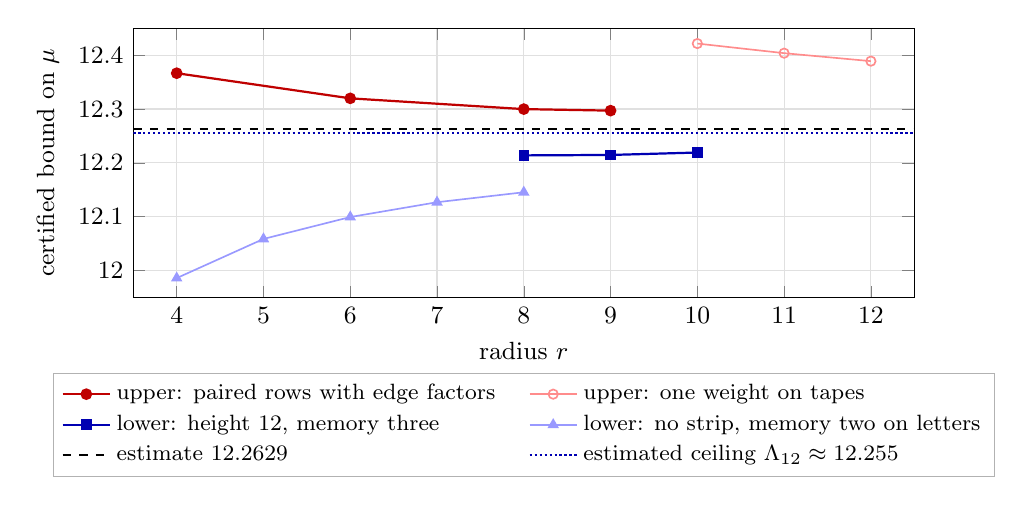
\begin{tikzpicture}
\begin{axis}[width=11.5cm,height=5.0cm,xlabel={radius $r$},ylabel={certified bound on $\mu$},
  xmin=3.5,xmax=12.5,ymin=11.95,ymax=12.45,grid=major,grid style={black!12},
  ytick={12.0,12.1,12.2,12.3,12.4},yticklabel style={/pgf/number format/fixed,/pgf/number format/precision=1},
  legend style={at={(0.5,-0.28)},anchor=north,font=\footnotesize,draw=black!30,legend columns=2,
    /tikz/every even column/.append style={column sep=1em}},legend cell align=left,
  tick label style={font=\small},label style={font=\small}]
\addplot[mark=*,mark size=1.7pt,line width=0.8pt,red!75!black] coordinates
  {(4,12.366448572318)(6,12.319749766858)(8,12.299756359)(9,12.296933854)};
\addlegendentry{upper: paired rows with edge factors}
\addplot[mark=o,mark size=1.7pt,line width=0.6pt,red!45!white] coordinates
  {(10,12.421514463859)(11,12.403654977316)(12,12.388844617135)};
\addlegendentry{upper: one weight on tapes}
\addplot[mark=square*,mark size=1.5pt,line width=0.8pt,blue!70!black] coordinates
  {(8,12.213777757442)(9,12.214596070132)(10,12.219100857094)};
\addlegendentry{lower: height 12, memory three}
\addplot[mark=triangle*,mark size=1.8pt,line width=0.6pt,blue!40!white] coordinates
  {(4,11.985857574)(5,12.058577430)(6,12.099279121)(7,12.126797697)(8,12.145297924)};
\addlegendentry{lower: no strip, memory two on letters}
\addplot[dashed,line width=0.7pt,black] coordinates {(3.5,12.262874)(12.5,12.262874)};
\addlegendentry{estimate $12.2629$}
\addplot[densely dotted,line width=0.8pt,blue!70!black] coordinates {(3.5,12.255)(12.5,12.255)};
\addlegendentry{estimated ceiling $\Lambda_{12}\approx12.255$}
\end{axis}
\end{tikzpicture}
\caption{Certified bounds by radius: paired upper certificates, earlier single-weight upper certificates, the stages
of Table~\ref{tab:lower} (last stage only at radius $10$), and earlier flows without a strip. The dotted line is an
extrapolated estimate of $\Lambda_{12}$, which caps every lower bound on the strip of height $12$.}
\label{fig:radius}
\end{figure}

\subsection{The upper bound}

\emph{Many rows are nearly tight.} The optimized certificate is a plateau: a large share of the formal rows have row
values close to the maximum. At the radius-$8$ certificate, $45$ percent of the groups of formal rows related by
reflection lie within $10^{-4}$ of the largest row value, and $53$ percent after a longer optimization; only $218$
groups lie within $10^{-5}$. So the bound is not held up by a few bad rows that a local repair could fix. The nearly
tight rows are the typical ones: the numbers of $+$ and $-$ in the row differ by $1$ or $3$, the signs change often,
and the run of equal letters at the head is short. Rows with a large imbalance or long runs have slack above $0.01$,
that is, their row values are at least $0.01$ below the maximum.

\emph{No unused freedom in the family.} Every kind of edge already carries a factor, and each part of the weight
already reads as far as the formal row allows, so within the family only a longer row helps. Adding weight factors
that count letters or sign changes beyond the row changes the bound by less than $10^{-5}$. Adaptive refinement of the
tables gets $82$ percent of the gain of the next radius from half of its new table entries, but does not reduce the
number of formal rows to check.

\emph{Cost and projection.} The number of formal rows grows fourfold per unit of radius. The radius-$9$ run was stopped
before it converged, still gaining about $10^{-4}$ per ten minutes. Extrapolating the converged optima at radius $4$,
$5$, $6$ and $8$ suggests about $12.2935$ for the radius-$9$ family and $12.289$ at radius $10$: less than $0.01$ per
step, at four times the cost. This is an extrapolation, not a bound.

\subsection{The lower bound}

\emph{The strip caps the bound.} Every flow on the strip of height $12$ gives at most $\Lambda_{12}$, the growth rate
of meanders whose labels stay in $-6\le g\le6$. Extrapolation from heights $2$ to $8$ puts $\Lambda_{12}$
near $12.255$ (plausible range $12.245$ to $12.261$), $\Lambda_{10}$ near $12.239$ and $\Lambda_{14}$ near $12.260$.
The cap does not limit the present bound, but it will once the radius and the family improve enough.

\emph{The radius and the family.} The best bound from any flow at radius $10$ and height $12$, not only from flows
of the form used here, is estimated at $12.22$ to $12.24$. At small size the four-move cycles span only $54$ to $57$ percent of the stationary directions; walks of six
and eight moves recover part of the rest. The last two increments of $131{,}072$ directions gained $0.00186$ and
$0.00076$.
% UNVERIFIED: "about 0.0003" for a third increment is a one-ratio guess in 1228; not quoted.
The next steps, in the order the computations suggest, are more complete stationary directions with a joint
optimization of all coefficients, a reference law optimized at the radius of the certificate, and then height $14$.
An exact parent at radius $7$ could not be computed within $3$~GB of memory and $45$ minutes.

\subsection{Summary}

Both methods see a bounded neighborhood of the head, and both gaps to the estimate close only as fast as that
neighborhood grows. We found nothing that changes this rate. Proving $12.26\le\mu\le12.27$ would need the lower bound to gain about $0.041$,
beyond the estimated cap of height $12$, and the upper bound about $0.027$.


\clearpage
\appendix
% Appendix A. Folder map; statuses from the FINAL.md of each folder, ledger/STATE.md and the wave-1200 handovers.
%%%%%%%%%%%%%%%%%%%%%%%%%%%%%%%%%%%%%%%%%%%%%%%%%%%%%%%%%%%%%%%%%%%%%%%%
\section{Where the proofs are}\label{app:where}
%%%%%%%%%%%%%%%%%%%%%%%%%%%%%%%%%%%%%%%%%%%%%%%%%%%%%%%%%%%%%%%%%%%%%%%%

Paths are relative to the directory \path{meandric/research} of the project repository~\cite{Repo}. ``Read
independently'' means that a separate reading, in the folder named, wrote its own proof or its own checking program.
Nothing has been reviewed outside the project. Files larger than about $50$~MB, among them the upper witness and the
two last lower increments, are kept on external storage and referenced from their folders by name and SHA-256 hash.

Three numbers to reproduce first with a new implementation: the closed walks of Theorem~\ref{thm:tape} give
$1,2,8,42,262,1828,13820,110954$; the upper certificate gives the largest row value $R_+$ with
$R_+^2=12.29693385352921289818\ldots$; the final lower stage gives the entropy bound $h\ge1.2515001857$.

\begin{table}[H]
\centering
\scriptsize
\setlength{\tabcolsep}{3.5pt}
\renewcommand{\arraystretch}{1.08}
\begin{tabular}{>{\raggedright\arraybackslash}p{3.4cm}>{\raggedright\arraybackslash}p{7.6cm}>{\raggedright\arraybackslash}p{4.0cm}}
\toprule
result & where & status \\
\midrule
Stack rules (label machine); Lemma~\ref{lem:labels} &
\path{630_referee_band_growth/REPAIRS.md}, section~2 (Lemma~1, Theorem~M); also \path{607_bounds_paper/paper_word.tex}, Appendix~A &
proved; read independently \\
Theorem~\ref{thm:tape} (tape machine) &
\path{637_rung2_matrix_product/PROOF.md}, section~1 (Proposition~T); review in \path{677_tape_bijection_review} &
proved; read independently; counts to $n=9$ (\path{1251}) and $n=15$ (\path{1252}) \\
Lemma~\ref{lem:sweep} (linear completion) &
\path{805_entropy_certificates/PROOF.md}, section~1.2, step~3; \path{641_tape_window_bounds/PROOF.md}, Lemma~R &
proved; read independently (\path{808}) \\
\addlinespace
Lemma~\ref{lem:oneweight} (one weight) & \path{641_tape_window_bounds/PROOF.md}, Lemma~U & proved \\
Lemma~\ref{lem:paired}, Corollary~\ref{cor:paired}; head and edit factors &
\path{1003_paired_path_consistency/PROOF.md}, sections~1--3; \path{1007_edit_edge_1230/PROOF.md} &
proved; re-proved independently (\path{1251_referee_upper_12297}) \\
Lemma~\ref{lem:local}, Proposition~\ref{prop:rows} &
\path{1201_upper_structures/PROOF.md}; \path{641_tape_window_bounds/PROOF.md}, section~2 &
proved; re-proved, sharpness tested (\path{1251}) \\
Upper certificate (Table~\ref{tab:upper}) &
\path{1201_upper_structures/runs/r9_run2_cand.json} (SHA-256 \texttt{332b0346\ldots2246}), report \path{r9_run2_verify.json}; checker \path{1007_edit_edge_1230/verify.py} &
certified (exact); independent exact checker in \path{1251} \\
\addlinespace
Lemma~\ref{lem:region} (finite region) & \path{641_tape_window_bounds/PROOF.md}, Lemma~L & proved \\
Theorem~F, memory two on letters & \path{805_entropy_certificates/PROOF.md}, section~1 & proved; read independently (\path{808_referee_flow_bound}) \\
Theorem~F on strips, memory $m$; closed walks, signed parent, sparse refinement &
\path{1019_overnight_structural} (\path{MEMORY_THREE_EXTENSION.txt}, \path{SIGNED_PARENT_CERTIFICATE_ARGUMENT.txt}, \path{SPARSE_CONTEXT_REFINEMENT_ARGUMENT.txt}); \path{1008_lower_122/PROOF.md}; written out in \path{1252_referee_lower_theory/PROOF.md} &
proved; re-derived independently (\path{1252}) \\
Lower certificate (Table~\ref{tab:lower}); reference law &
\path{1228_combined_lower/inc2_131072_certificate.json}, \path{verify_cmd.sh}; earlier stages in \path{1204_coarse_coordinates/data/alt7}; law \path{1019_overnight_structural/memory_three.py} &
certified (exact, outward rounding); recomputed independently (\path{1253_referee_lower_computation}); later audit in \path{1426_audit_paperB_lower}; portable format in \path{1421_export_lower_certificate/SPEC.md} \\
\addlinespace
Plateau, projection $12.289$; ceilings $\Lambda_K$ & \path{1201_upper_structures/FINAL.md}; \path{1203_ceiling_ladder/FINAL.md} & numerical; projections are conjectures \\
Strip of three levels & \path{630_referee_band_growth} & proved; read independently \\
Other certificates in Figure~\ref{fig:radius} & \path{1007_edit_edge_1230}, \path{1201} (paired); \path{641_tape_window_bounds} (one weight); \path{809_flow_certificate_scaling} (no strip) & certified (exact) \\
\bottomrule
\end{tabular}
\end{table}


\bibliographystyle{plain}
\bibliography{../common/refs}

\end{document}
